\newcommand{\YEAR}{2015}
\newcommand{\SEMESTER}{FS \YEAR}
\newcommand{\SUBTITLE}{Untertitel}
\newcommand{\DATE}{{\today}}
\newcommand{\TITLE}{Functional Kafka}
\newcommand{\AUTHOR}{Marc Juchli, Lorenz Wolf}
\newcommand{\SUPERVISOR}{Prof Dr. Josef Joller}
\newcommand{\EXPERT}{Dr. Simon Meier}
\newcommand{\EMAIL}{\{l1wolf, mjuchli\}@hsr.ch}
\newcommand{\KEYWORDS}{Bachelor Thesis, Computer Science, HSR, \SUBTITLE, \TITLE}

\documentclass[11pt,oneside,a4paper,parskip,listof=numbered]{scrreprt}
\usepackage[inner=2.5cm,outer=2cm,top=2cm,bottom=2cm,includefoot]{geometry}

\usepackage{cmbright}
\setlength{\parindent}{0pt}
\setlength{\parskip}{6pt plus 2pt minus 1pt}
\setlength{\emergencystretch}{3em}  % prevent overfull lines

\usepackage[T1]{fontenc}
\usepackage[utf8]{inputenc}
%/usepackage{ngerman}
\usepackage{graphicx}
\usepackage{color}
\usepackage{ccicons}
\usepackage{rotating}
\usepackage[colorlinks=true, linkcolor=blue, urlcolor=blue, citecolor=blue]{hyperref}
\usepackage{pdfpages}
\usepackage{todonotes}
\usepackage{tabularx}
\usepackage{xcolor,colortbl}
\usepackage{pdflscape}
\usepackage{soul}
\usepackage{glossaries}
\usepackage{amsmath}
\usepackage{amssymb}
\usepackage{pifont}
\usepackage{fourier}
\usepackage{MnSymbol}
\usepackage{wasysym}
\usepackage{float} % Bilder fix positionieren
\usepackage{appendix}
\usepackage{booktabs}
\usepackage{makeidx}
\makeindex
\usepackage{fancybox}
\usepackage[nottoc,numbib]{tocbibind}
\usepackage{enumitem}
% \usepackage{slashbox} %halbierte Tabellenzellen
% \setlist{nolistsep}
\setlist[itemize]{noitemsep, topsep=0pt}

\usepackage{tikz}
\usepackage{pgf-umlsd}
\usepgflibrary{arrows} % for pgf-umlsd

% \let\stdsection\section
% \renewcommand\section{\newpage\stdsection}

\subject{\SUBTITLE}
\title{\TITLE}
\author{\AUTHOR \\ \EMAIL}

\hypersetup{
  pdftitle    = {\TITLE},
  pdfsubject  = {\SUBTITLE},
  pdfauthor   = {\AUTHOR, \EMAIL},
  pdfkeywords = {\KEYWORDS} ,
  pdfcreator  = {pdflatex},
  pdfproducer = {LaTeX with hyperref}
}


\newcommand{\logoLX}{\fcolorbox{white}{red}{\textcolor{white}{LX}}}
\newcommand{\logoSH}{\fcolorbox{white}{maroon}{\textcolor{white}{SH}}}
\newcommand{\logoSE}{\fcolorbox{white}{orange}{\textcolor{white}{SE}}}
\newcommand{\logoXJ}{\fcolorbox{white}{darkblue}{\textcolor{white}{XJ}}}
\newcommand{\logoXC}{\fcolorbox{white}{darkgreen}{\textcolor{white}{XC}}}
\newcommand{\logoMF}{\fcolorbox{white}{lila}{\textcolor{white}{M4}}}
\newcommand{\logoMS}{\fcolorbox{white}{violett}{\textcolor{white}{M6}}}
\newcommand{\logoMN}{\fcolorbox{white}{pink}{\textcolor{white}{MN}}}

\newcommand{\verwundbar}{\hfill \fcolorbox{black}{red}{(Verwundbar \bomb)}}
\newcommand{\nichtverwundbar}{\hfill \fcolorbox{black}{green}{(Nicht verwundbar~\sun)}}
\newcommand{\zelleverwundbar}{\cellcolor{red} \bomb}
\newcommand{\zellenichtverwundbar}{\cellcolor{green} \sun}
\newcommand{\zelleteilweiseverwundbar}{\cellcolor{yellow} \danger }
\newcommand{\gegenmassnahme}{$\rightarrow$ Die Gegenmassnahme ist in diesem Kapitel zu finden: }
\newcommand{\keinegegenmassnahme}{$\rightarrow$ Diese Verwundbarkeit lässt sich mit keiner Gegenmassnahme beheben.}

\definecolor{yellow}{RGB}{240,173,78}
\definecolor{orange}{RGB}{255,128,0}
\definecolor{lila}{RGB}{128,128,192}
\definecolor{violett}{RGB}{64,0,128}
\definecolor{pink}{RGB}{255,128,192}

% Code-Listing
\definecolor{gray}{rgb}{0.4,0.4,0.4}
\definecolor{darkblue}{rgb}{0.0,0.0,0.6}
\definecolor{cyan}{rgb}{0.0,0.6,0.6}
\definecolor{green}{RGB}{92,184,92}
\definecolor{red}{RGB}{217,83,79}
%\definecolor{light-gray}{gray}{0.95}
%\definecolor{lbcolor}{rgb}{0.9,0.9,0.9}
\usepackage{listings}
\definecolor{maroon}{rgb}{0.5,0,0}
\definecolor{darkgreen}{rgb}{0,0.5,0}
\definecolor{sh_comment}{rgb}{0.12, 0.38, 0.18 } %adjusted, in Eclipse: {0.25, 0.42, 0.30 } = #3F6A4D
\definecolor{sh_keyword}{rgb}{0.37, 0.08, 0.25}  % #5F1441
\definecolor{sh_string}{rgb}{0.06, 0.10, 0.98} % #101AF9

% \lstset{numbers=left,
%     language=Java,                               % oder C++, Pascal, {[77]Fortran}, ...
%     basicstyle=\ttfamily,                        % Textgröße des Standardtexts
%     keywordstyle=\ttfamily\color{red},           % Formattierung Schlüsselwörter
%     commentstyle=\ttfamily\color{green},         % Formattierung Kommentar
%     stringstyle=\ttfamily\color{blue},           % Formattierung Strings
%     breaklines=true,                             % Umbruch langer Zeilen
%     showstringspaces=false,                      % Spezielles Zeichen für Leerzeichen
% }
\lstset {
 frame=rlbt,
 rulesepcolor=\color{black},
 showspaces=false,showtabs=false,tabsize=2,
 %numberstyle=\tiny,numbers=left,
 basicstyle=\ttfamily\footnotesize,
 stringstyle=\color{sh_string},
 keywordstyle = \color{sh_keyword}\bfseries,
 commentstyle=\color{darkgreen}\itshape,
 captionpos=b,
 %lineskip=-0.1em,
 showstringspaces=false,
 escapebegin={\lstsmallmath}, escapeend={\lstsmallmathend},
 breaklines=true, % breakatwhitespace=true,
 prebreak=\raisebox{0ex}[0ex][0ex]{\ensuremath{\rhookswarrow}},
 % postbreak=\raisebox{0ex}[0ex][0ex]{\ensuremath{\rcurvearrowse\space}}
}
\lstnewenvironment{code}{\lstset{language=Haskell}}{}

\newcommand{\inputlisting}[2][]{%
  \lstinputlisting[caption={\texttt{\detokenize{#2}}},#1]{#2}%
}

\lstdefinelanguage{XML}
{
  basicstyle=\ttfamily\footnotesize,
  morestring=[b]",
  moredelim=[s][\bfseries\color{maroon}]{<}{\ },
  moredelim=[s][\bfseries\color{maroon}]{</}{>},
  moredelim=[l][\bfseries\color{maroon}]{/>},
  moredelim=[l][\bfseries\color{maroon}]{>},
  morecomment=[s]{<?}{?>},
  morecomment=[s]{<!--}{-->},
  commentstyle=\color{darkgreen},
  stringstyle=\color{blue},
  identifierstyle=\color{red}
}

\makeglossaries
\chapter{Glossar}

\begin{description}
  \item[Artifact] Gegenstand
  \item[Socket] Communication endpoint to which an application can write data
that are to be sent out over the underlying network, and from which incoming end
data can be read. \cite{TAN06}
\end{description} 



\begin{document}
\begin{titlepage}
\begin{flushleft}

\begin{center}
\begin{minipage}[t]{0.45\textwidth}
  
\includegraphics[width=\textwidth]{images/hsr_logo.pdf}
\end{minipage}
\begin{minipage}[t]{0.45\textwidth}
 
\includegraphics[width=\textwidth]{images/haskell_kafka_logo.pdf}
\end{minipage}
\end{center}
\noindent\begin{minipage}[t]{0.49\textwidth}
  \begin{flushleft}
    \vspace{0pt} %needed else aligned to bottom
    % 
\includegraphics[width=1\textwidth]{images/hsr_logo.pdf}
  \end{flushleft}
\end{minipage}
\hfill
\begin{minipage}[t]{0.49\textwidth}
  \begin{flushright}
    \vspace{0pt} %needed else aligned to bottom
  \end{flushright}
\end{minipage}
\\[4cm]

{\huge \bfseries \TITLE}\\[2.5cm]
% {\large \bfseries \SUBTITLE}\\[2cm]

Bachelor Thesis \\
\SEMESTER \\
Computer Science Department \\
HSR - University of Applied Sciences Rapperswil \\
\url{http://www.hsr.ch/}\\[2cm]


\vfill

Authors: \AUTHOR \\
Supervisor: \SUPERVISOR \\
Expert: \EXPERT \\
Scope of work: 12 ECTS (360 hours of work per Student) \\
Duration: February 16 until June 12, 2015 \\
% Datum: {\DATE}

\end{flushleft}
\end{titlepage}

\hypersetup{linkcolor=black}
\setcounter{tocdepth}{1}

\begin{abstract}
 Abstract here
\end{abstract}


\tableofcontents

\part{Introduction}
\chapter{Management Summary}

\section{Introduction}

This thesis aims to adapt the concept of Apache Kafka and build a messaging
system, namely Haskell Message Broker (HMB), in the functional programming
language Haskell. Thereby the focus lies on the implementation of a stable
(related to networking) server application system as well as on the building a
log subsystem, which in Apache Kafka is considered to be the most important
feature. As Kafka comes with its own wire-protocol a part of this thesis will
focus on a fully compatible implementation of the Apache Kafka Protocol in
Haskell, including a client library allowing Haskell applications to take use of
the protocol implementation and communicate with Apache Kafka or HMB.

\section{Approach}

First of all we started to become familiar with the state of the art in
messaging, especially event streaming. As essential part of this prestudy we
analysed the approach and functionality of Apache Kafka. In this first third of
the thesis we also learned the functional paradigm and the programming language
Haskell intensively. After the prestudy phase we elaborated an architecture prototype
to demonstrate some very basic functionality of a message broker. We then
followed by working out the details for the protocol implementation and the
server application. A code review by expert Simon Meier helped us to tweak our
code and improve efficiency. Finally, we tested our system under high load to
optimize performance of our application.

\section{Results}

The first result of this thesis is the prestudy documentation, which
resumes gathered knowledge in the familiarization phase of this work.
It gives an insight in messaging fundamentals and  takes a closer look to Apache
Kafka and related topics. It can be offered for using as academic amendment for
existing lectures. Another result is the implementation of the Kafka protocol in
Haskell. The design decision of separating protocol related code from the broker
implementation leads to a isolated product which can be used as library for
different projects. The open sourced code has already been praised by the
Haskell community and found its contributors helped uncovering minor
issues. Finally, the resulting broker application provides a server
with basic functionality in networking and persisting messages. It adapts
some features of Apache Kafka and provides the ability to produce and consume
data. It supports Kafka clients as it is based on the protocol implementation
mentioned above. Simple console clients are provided to demonstrate the
functionality.

\section{Outlook}

- broker results promissing
- very extendable/scalable implementation base and architecture
- with further work one could build the current prototype to an extraordinary
broker system.

As for now, the highlight remains the protocol implementation which has already
been praised by the Haskell community and found its contributors they helped
uncovering minor issues.

\chapter{Task Description}
(by Josef Joller)

\chapter*{Declaration of Authorship}
We declare that this bachelor thesis and the work presented in it was done by
ourselves and without any assistance, except what was agreed with the
supervisor or expert. All consulted sources are clearly mentioned and cited correctly. No
copyright-protected materials are unauthorizedly used in this work.

\hfill \\
\hfill \\

\begin{tabular}[l]{p{7cm} p{7cm}}
   Rapperswil, ...........................
   & ......................................... \\
   & Marc Juchli \\
   &\\ & \\
   Rapperswil, ...........................
   & ......................................... \\
   & Lorenz Wolf \\
   &\\ & \\
\end{tabular}




\part{Technology Research}
\chapter{Motivation} 

In distributed systems and the involved technologies, a significant amount of
terms and definitions have been given in the literature. First part of this
preparatory study aims to achieve more clarity in this confusing and oftentimes
ambiguous \textit{jungle of terminology}, whereas the focus lies on topics that
are related to Apache Kafka. After defining basic concepts for referencing
during this thesis, we go deeper into the technology and components of Apache
Kafka itself. Finally we compare other implementations of similar systems
whereas the goal of this survey is to uncover the differences of the most
related alternatives in contrast to Apache Kafka. \\

\begin{figure}[H]
    \centering
    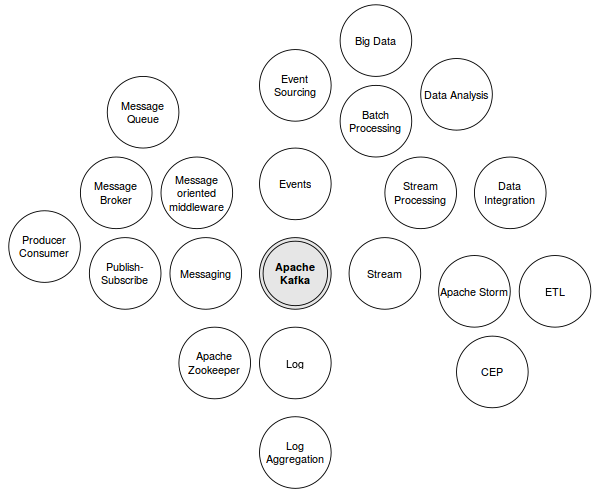
\includegraphics[width=0.6\textwidth]{images/jungle-of-terminology.png}
    \caption{\textit{Jungle of Terminology} related to Apache Kafka}
    \label{fig:jungle-of-terminology}
\end{figure}


\chapter{Introduction to Messaging} 

\section{Message Oriented Middleware}
\label{intro-messaging-mom}
Introducing an intermediate component between distributed
clients, messaging reduces the close coupling of other communication styles just
based on \gls{Socket}s or RMI. This additional component can be named as
Message-Oriented Middleware (MOM) and is all about passing \gls{Msg}s in any
format from one application to another whereas the parties do not need to know
each other directly. Thereby the main characteristic of a MOM is that its
supports a storage capacity which leads to a persistent way of communication where it is
not required that the collaborating endpoints are active during the entire
transmission of a message. This loose coupling in time is achieved by
working with queues as data structure (first-in-first-out) where applications
can insert their messages and a receiver program can read from this queue at a
different time. In normal case the original sender
never has the guarantee that the sent message has arrived at the desired
destination but it always has the confirmation of the MOM that the data has put
in a message queue. \cite{PprIBMIntro} \cite{TAN06}

\section{Interoperablity}
Because its interoperability, messaging is a very interesting communication
style for enterprise integration. Basically interoperability means that system with
different technologies can collaborate together by using the same standard or
protocols. While using a messaging system in an enterprise environment it is
much more efficient to integrate a new application to the existing data flow.
Instead of implementing a new interface for another technology, the additional
software can be just linked to the existing MOM by using the underlying
messaging protocol.\\

In the past, several companies like IBM or Microsoft developed their own
proprietary standards and protocols for asynchronous messaging systems.
Probably to keep it locked in their customer base. In June 2001 the Java Message
Service API (JMS) was released as best-known standard for messaging systems.
However, it is only an interface an not a specific protocol, JMS implementations
need to define their own. There was still no general protocol standard which
would have allowed to interoperate between different messaging implementations.
Fortunately in June 2006 a pool of multiple companies for network technologies
defined the Advanced Message Queueing Protocol (AMQP) as a open standard for an
interoperable messaging protocol. \cite{PrpAMQP}
 
%\begin{description} 
%	\item [Advanced Message Queuing Protocol (AMQP)] \hfill
%    \item [JMS]	
%\end{description}

\section{Point-To-Point Connection}
\label{intro-messaging-pointtopoint}
A Point-To-Point connection is the simplest architecture for communicating in a
messaging system. In a very basic scenario with a node A as sender of a message
and a node B as receiver, the MOM (running either on the node itself or
dedicated in the local network) assumes the task of handling a local queue for messages and manages an address-lookup
database for mapping destination names to network locations. The sender puts its
message in his local queue whereas the MOM organises the network transfer to the
queue of the target. In turn the receiver system can read from its own
local queue the incoming message. The MOM provides a specific API for both the
sender as well for the receiver:
\begin{table}[H]
\centering
\begin{tabular}{|l|l|}
\hline
\textbf{Put}    & Append a message to a specific queue                                        \\ \hline
\textbf{Get}    & Block until the specific queue is nonempty, and remove the first message    \\ \hline
\textbf{Poll}   & Check a specific queue for messages, and remove the first                   \\ \hline
\textbf{Notify} & Install a handler to be called when a message is put into a specified queue \\ \hline
\end{tabular}
\caption{Basic API for message queue implementation \cite{TAN06}}
\end{table}

This kind of communcation works well in an environment with two systems which
want to collaborate and use the advantages of messaging. But if there are more
than two nodes, the local mapping of a queue name to a foreign network location
implies that each system needs to hold the addresses of all the other nodes that it
wants to communicate with. When a target address changes, all the systems that
communicate with the target must be updated. In most scenarios there is also a need
for transforming messages in different format where these implementations have
to be made on every node, which leads to duplicating code.  For more complex
integration solutions, a centralised solution whereas the MOM runs on a location
independent platform is required. This is where the message broker comes into
game. \cite{MSDNIntegration}

\section{Message Broker}
\label{intro-messaging-broker}
A messaging system with point-to-point connections can decouple two systems
by using a managed queue on each side of a collaboration. But there is
still the need of configuration the endpoints on each party. In general, a
message broker is a dedicated component which decouples source and
target systems by assuming full responsibility for coordinating communication between
all connected nodes. Thereby the main tasks of a message broker are the
dynamically registration of endpoints, determining location of target system
(a.k.a. routing) and performing of the communication as well transformation of a
message from one format to another.\cite{MSDNIntegration} \\

\subsection{Broker Pattern}
As initial point for the detailed definition of a message broker we take the
\textit{Broker Pattern} of  \textit{Patterns of Software Architecture Volume1}
which can be used to structure distributed systems with decoupled components.
Basically it differs between two types of brokers, where the \textit{Direct
Broker} performs a initialization of a connection but the following communication
is only between the two endpoints. For messaging, the second variant
\textit{Indirect Broker}, is lot more interesting because it maintains all of
the communication between the nodes at every time. So let us define the message
broker as refinement of the Indirect Broker Pattern for message-based
communication.\cite{POSA1} 

%\subsection{Structure}
The \textit{Broker Pattern} consists of five types of participating components,
which we can adapt for a message based environment by using the common terms.

\begin{description}
    \item[Producer (adapted from Client component)] \hfill \\
        {Applications that either generating data for later processing or
        accessing a service from another client in the messaging system. In both
        cases the producer pushes its messages to the broker and in general don't care 
        about it anymore.}
    \item[Producer API (adapted from Client-Side-Proxy)] \hfill \\
        {Structural component which encapsulates messaging-specific
        functionality from the rest of the client code. Thereby, a call from the producer
        can be transformed to a message in the right format. The producer API
        directly communicates with the broker API.}
    \item[Broker] \hfill \\
        {Central component that acts as a mediator and is responsible for the
        transmission of messages from multiple producers to multiple consumers.
        A broker offers an API to the messaging clients, both for consumer and
        producer. It also must have kind of a directory for locating registered
        consumers.} 
    \item[Consumer (adapted from Server component)] \hfill \\
        {Basically the consumer is a endpoint which receives and processes a
            message for further activities. An \textit{Event-Driven-Consumer}
            handles incoming messages automatically as they are pushed from the
            broker. A \textit{Polling-Consumer} explicitly gets messages when it
            wants to receive it from the broker. If a consumer provides a
            service to other clients, it also can act as a producer for sending
            back messages as response.}
\item[Consumer API (adapted from Server-Side-Proxy)] \hfill \\
        {Structural component which encapsulates messaging-specific
        functionality from the rest of the client code. Based on incoming
        messages it calls services within the consumer component. }
\end{description}

\begin{figure}[H]
    \centering
     \begin{sequencediagram}
        %\newthread{broker}{Broker}
         \newinst[1]{producer}{Producer}
         \newinst[1]{producerProx}{Producer API}
         \newinst[1]{broker}{Broker}
        \newinst[1]{consumerProx}{Consumer API}
        \newinst[1]{consumer}{Consumer}
        \begin{messcall}
            {producer}{(1) Send Request}{producerProx}{}
        \end{messcall}
        \begin{call}
            {producerProx}{(2) Pack data}{producerProx}{}
        \end{call}
        \begin{messcall}
            {producerProx}{(3) Transmit message}{broker}{}
        \end{messcall}
        \begin{call}
            {broker}{(4) Find Consumer}{broker}{}
        \end{call}
        \begin{messcall}
            {broker}{(5) Deliver Message}{consumerProx}{} 
        \end{messcall}
        \begin{call}
            {consumerProx}{(6) Unpack Data}{consumerProx}{}
        \end{call}
        \begin{messcall}
            {consumerProx}{(7) Forward Message}{consumer}{}
        \end{messcall}
    \end{sequencediagram}
    \caption{General structure of the Broker Pattern with Event-Based
    Consumer}
    \label{fig:MB-SSD-1}
\end{figure}
%We saw that a \textit{Broker} acts like a mediator between to collaborating
%applications which do not need to know each other. The same does a message
%broker, of course in a message-oriented distributed system whereas the broker
%handles incoming messages from a source to a target and backwards.

%In such an environment it is essential that existing and new applications can be
%integrated into a single, coharent system at runtime. Often these applications
%are not speaking the same language and it need kind of a gateway for
%transforming messages into a format that can be unterstood by the receiver.
%\cite{TAN06}

%\subsection{Routing and Communicating}

%\subsection{Transformation}

\subsection{Characteristics}
As described a messaging system has its strengths in interoperability and louse
coupling of distributed computers. A message broker in turn has also many further
characteristic where we have described the most related to our work as follows:  

\begin{description}
    \item [Architecture] \hfill \\
    { A fundamental design decision for a message broker is whether consumers
    should pull data from brokers or brokers should push data to consumers. This
has direct impacts to the performance of a broker system whereas in a push-based
environment the consumers can be the bottleneck when its consumption rate falls
below the rate of production. In a pull-based system consumers which fall back
can catch up at any time whereas the risk of bottleneck lies at the broker thus
 a message broker should scale well. On the other hand in a pull-based
 environment a consumer never knows whether a message is ready for consumption
 or not. In worst case this ends up with a read loop where the consumer
 constantly need to check the queue. \cite{apachekafka} }
    \item [Delivery Reliability] \hfill \\
    {
    A reliable delivery of messages can promise a specific behaviour to producer
    and consumer. A message broker typically supports one ore more of the
    following guarantees.
    \textit{At most once} guarantees that messages may be lost but are never
    redelivered. \textit{At least once} is defined that messages are never lost
    but may be redelivered. The \textit{Exactly once} semantic which is very
    typical guarantees that each message is delivered only once. Broker system
    which use the \textit{In Order} semantic deliver messages to the consumer in
    the strict same order they are sent from the producer to the broker. 
    }
    \item [Independence] \hfill \\
    { Independence to specific technologies or systems. The more independent a
        message broker is, the better it can be integrated in a existing
        environment. The use of standards and effective standardized interfaces
        promotes independence.}
    \item [Scalability] \hfill \\
    {Ability to dynamically increase performance depending on work load.  }
    \item [Latency]\hfill \\
    {Elapsed time it takes to process a single message for consumption.  }
\item [Fault Tolerance] \hfill \\
        {Ability to recovery after a failure with minimal message loss.
        Possibility to build redundancy through clustering and replication strategy such as
        master slave\todo{gls} or state machine replication\todo{gls}. It is a significant
    characteristic how a message broker syncs its replications and decides which
    of the nodes to get active if the master fails. Also it is important that in case of
failure the system can recover as quickly as possible and with minimal
throughput deficit.   }
        \item [Persistency] \hfill \\ 
        {Ability to offer durable and persistent messages although the broker
            systems restarts, crashes or consumer is inactive for longer period of time
            (for instance batch processing system). }
    \item [Throughput] \hfill \\
        {Proportion of messages which can be sent to a broker to the amount of
        messages which can be consumed in a fixed time interval.}
\end{description}

\subsection{Publish / Subscribe Channel} 
Basically, a channel is equivalent to the managed queues we described so far. In
a channel one application can write messages and another one reads that
information from it. Because a message broker can handle multiple clients with
variable behaviour we can differ between different channel.a

Sending messages to the broker in form of publishing to a specific topic and on
the other hand receiving messages only for the specified topic, is called
publish/subscribe. In contrast to a one-to-one channel, the message broker
requires the abilities to match messages on an application based level to act as
a gateway for topic related messages. Based on the informations provided within
the messages, the broker is being able to provide the messages to the client
acting as a subscriber \cite{TAN06}. In fact, the publish/subscribe channel
delivers a copy of the topic related messages to the output channel. This also
means that there can be more than one client that consumes the topic specific
messages and thus there can be more than one subscriber. Especially this feature
of having multiple consumers of a message channel, is decisive for using a
message broker in environment where we want to process the same stream of
data in multiple ways. We will go in deeper detail to stream processing in the
following chapter. \cite{EIP03}

%\todo[inline]{Beschreibung und Sequenzdiagram: Consumer meldet sich für den
%Empfang beim Broker an } 


\chapter{Introduction to Event Streaming}

In previous chapter we defined what a message broker basically is, therefore we
can imagine how Apache Kafka works. Because Apache Kafka is build for big data
environments \todo{big data erklären} there is often mention of terms like Event or
Stream. When we want to understand what what Apache Kafka actually is for an
how it is used, we need to know what an Event Stream is.

\begin{figure}[H]
    \centering
    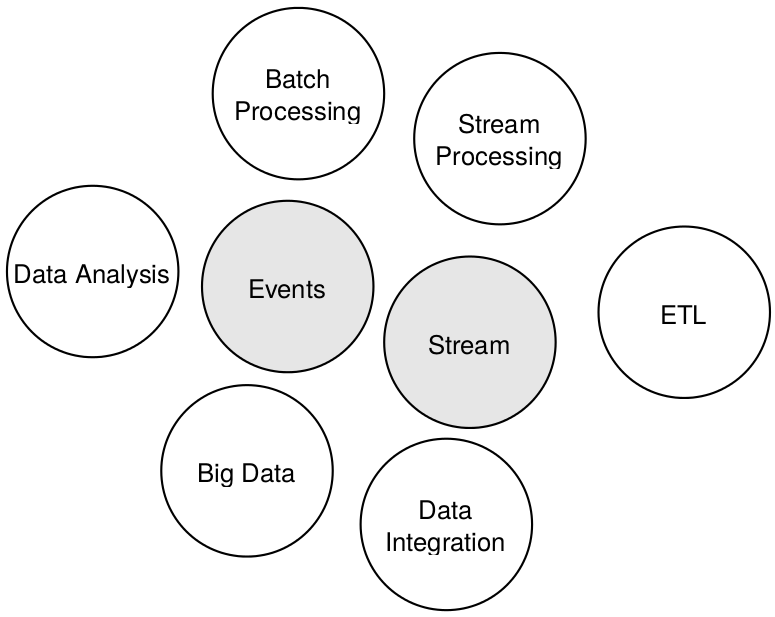
\includegraphics[width=0.45\textwidth]{images/evenstreaming-intro.png}
    \caption{Event Streaming terms}
    \label{fig:evenstreaming-intro}
\end{figure}

\section{Purpose}
The view of data as rows of databases or single files changes when one thinks
about what a business actually does with the generated data. Where retail
generates orders they lead to sales, shipments and so on, a financial
institution will generate orders they are going to have an impact of a stock
price. Or a social network platform generates clicks, impressions and searches
they are used to make some sort of intelligent analysis to further display
personalized data to it's users. Such kind of data can be thought of as streams
of events. In fact, collecting all events a business ever generated will lead to
the current state of the business and thus describe what the business did in
past. For example the current price of a stock was generated by all the orders
ever made on this stock. Every order can be captured as an event and so can all
events together reproduce the current stock price.

\section{What is an Event?}
\label{intro-datastream-datastream}
Very basically an event occurs when "something happens"  in a system like when a
user of an online shop adds an item to its basket. In modern systems, events are
transmitted as discrete messages on a MOM (see \ref{intro-messaging-mom}) and
thus following Tannenbaum et al. (2006), represent a data unit of a data
streams. Where a data stream can be applied to discrete as well as continuous
media, events are transmitted as discrete messages only. The message as itself
can be considered as an event message \cite{EIP03}.

If we think more traditionally, even database systems can be thought of as an
event based systems. The process of creating a backup in form of dumps won't
scale as we increase the frequency of dumps over time. Not only will the process
take longer according to the size of the database, also system resources are
limited during this process. An approach to make this more efficient \todo{why?}
is change capture, which describes the difference between the state of the
affected database rows before and after the change as event. If this can be done
continuously a sequence of row changes is what is being left. This in in fact,
can be described as a stream of events.

\section{Processing of Events}
Basically processing of events follows two key objectives: 
\begin{description}
    \item [Data Integration] \hfill \\ Making all the data of an organization available in all its services and systems.
    \item [Data Analytics]  \hfill \\ Preparing collected data for further analysis at any time. 
\end{description}

So data streams consisting of events as it self are not valuable but
can be taken advantage of by a system that processes these events, produces a
result and provide it to other services. This can be the calculation of the new
stock price after a customer sold his stock or the personalized content on a
news feed after a person subscribed to a new fan page. But it could also be a
more complex analysis over all the collected event that ever happened, stored in
a big database. 
\\ \\
In fact, the above mentioned examples differ in it's nature. Where the
calculation of the stock price is fairly simple by setting the price to the
latest paid stock price without any knowledge about the stock prices in past. 
In contrast, a complete analysis over a huge data base will not only require a
significant amount of processing time, it also requires some data produced in the
past. This leads to two different approaches to handle an incoming event stream
of any size: 

\begin{description}
    \item[Store raw data]  \hfill \\
    {Simply storing every single event in a big data store. Through appending
    every incoming event one get a wide history of every activity on the system.
    To analyze the data, a periodic batch process can execute big queries over
    all events to get a result.  $ \Rightarrow $  \textbf{Batch Processing}}
    \item[Store aggregated data  ] \hfill \\
    {Instead of persist every single event, directly process the incoming data stream and store
    only an aggregated summary. Because of updating the aggregation with every
    incoming event, getting an overall result is very fast (what we call
    "Real-Time"). Of course there is not a history of all the "happenings"
    anymore. $ \Rightarrow $ \textbf{Stream Processing}} 
\end{description}
\cite{TalkKleppmann}


\subsection{Batch Processing}
\label{intro-datastream-batchprocessing}
Traditional batch processing systems nowadays are distinguished between
map-reduce based and non map-reduce based systems 
\todo{cite} 

The process of  data integration (a.k.a data extraction-transformation-load, ETL
\todo{glossary}), runs at a regular time interval, such as daily, weekly or
monthly. Analyzing data that resides in a data store stage and becomes
challenging when data size grows and systems may not be able to process results
within a time limit. \cite{Liu:2014:SRP:2628194.2628251}

%\subsection{Real-time Batch Processing}
As the trend shows, the needs of performance and responsiveness in a big data
environment can't be fulfilled with traditional batch processing anymore.
Instead, real-time processing becomes more important than ever to achieve
results from queries in minutes, even seconds. 
\cite{bange2013big}

In real-time batch processing fashion, systems will address the data integration stage
with continual input of data. Processing in near-real-time [glossar] to present 
results within seconds is being addressed in data analytics. Thus,
real-time batch processing gives organization the ability to take immediate action
for those times when acting within seconds or minutes is significant.
\cite{PrpSvyOfDSPS}


\subsection{Stream Processing}
\label{intro-datastream-streamprocessing}
Stream processing refers to integration and processing of data before storing. 
A stream processing system is built out of multiple units called a processing
element (PE). Each PE receive input from their input queues, does some
computation on the input using its local state and produce output to their
output queues. PE communicate always through messaging with other PEs. 
\\ \\
Most important, those systems are optimized for high latency and high
availability. Recovering from failures is critical for a stream processing
systems and should be fast and efficient. 
Data should partitioned and handled in parallel for large volumes of data. 
The partitioning strategy of a system  affects how the system
handles the data in parallel and how the system can scale. 
\cite{PrpSvyOfDSPS}
\\ \\
Stream processing frameworks---such as Storm, Samza, or Spark
Streaming---were especially developed to provide rich processing primitives and
thus can be taken advantage of in the data integration- and processing stages.

\subsection{Other Terminology}
\subsubsection{Complex Event processing (CEP)}
In literatur there is often a confusion about the difference between
complex event processing and stream event processing. Both systems work on
events and produce results based on the properties of the events... 
- Zitat: Combines data from multiple sources  to detect patterns and attempt to
identify either opportunities or threats. The goal is to identify significant
events and respond fast. Sales leads, orders or customer service calls are
examples.\\

\todo[inline]{incomplete}

\subsubsection{Event Sourcing}
\label{event-sourcing}
Regarding to event processing we often met the term \textit{Event Sourcing} in
literature. It is a pattern originally defined by Martin Fowler which basically
treats with the same objectives as we mentioned for batch processing just with
other terms of the Domain-Driven-Design community. Instead of storing aggregated
data which represents the current state, the basic idea is to capture
every state change of an application as immutable event object. For later
analysis, this gives much richer information than just overwriting it. \todo{cite}

\section{Lambda Architecture}
While batch processing is used for data analysis to get results out of huge
amount of raw stored data at any time, stream processing reacts to events in
real time. Both approaches are very useful in different use cases. Lambda
architecture is a data-processing architecture designed to handle massive
quantities of data by taking advantage of both batch and stream processing
methods. It is split into three layers, the batch layer, the serving layer and
the speed layer:

\begin{figure}[H]
    \centering
    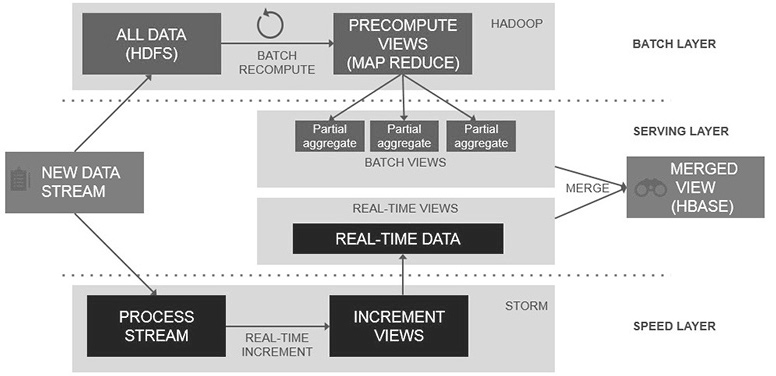
\includegraphics[width=1.0\textwidth]{images/lambda-architecture.jpg}
    \caption{Lambda Architecture}
    \label{fig:lambda-Architecture}
\end{figure}

Any query is answered through the serving layer by querying both the speed and
the batch layer. Where the badge layer periodically computes views on the
current collected data and is being outdated at the end of it's computation, the
speed layer closes this gap by constantly processing the most recent data in
near real-time fashion. \cite{marz2015big} \cite{PrpSvyOfDSPS}

\section{Centralized Event Stream}
\subsection{Need for a common data stream}
Any system which is dependent on a continuous input of data, requires a delivery
system that can provide data constantly as stream (can be
compared to an ordered message queue \todo{ref} containing events). Stream
processing systems, whether being in a lambda architecture or not, obviously
holds this requirement. On the other hand, in a big data environment there is
also the requirement of batch processing systems
(\ref{intro-datastream-batchprocessing}) being served with data. In a lambda
architecture this could be done using a stream processing framework
(\ref{intro-datastream-streamprocessing}) responsible for serving the batch
processing system with integrated data, ready for data analysis. However, an
other way of doing so would be a data store---such as the hadoop file system
(HDFS\todo{gls}---where data can be directly taken for further analysis.
The same requirement of a data store holds for any
other business intelligence system followed by the problem of the dependency of
a data store which eventually---due to the lack of an adapter---can not be
served with data by a stream processing system as comfortable as the HDFS.

\subsection{Requirements}
Facing the two types of processing events---stream- and batch
processing---together, data integration results as a common stage both system have to
deal with. Even further, for every system an organization operates, like the
data warehouse, full-text search indexes, caches or lot more, the data
integration stage will be present. 
Additionally, stream processing systems require a continuous
incoming stream to further integrate and process where batch processing systems
on the other hand demand a given persistent set of data to further integrate and analyze.

Further more, in terms of stream processing the requirement of low latency is
essential for any system of this type. For database systems combined with stream
processing, reliability becomes significantly important to handle critical updates 
such as replicating the as discussed above.
In terms of batch processing however, the demand on low latency is not as
important as the availability of well integrated data with a high throughput to
be able to handle a large volume of data in time range as low as possible.

\begin{table}[H]
\centering
\begin{tabular}{l|c|cl}
\multicolumn{1}{c|}{\textbf{}} & \textbf{Stream Processing} & \textbf{Batch
Processing} & \multicolumn{1}{c}{\textbf{}} \\ \cline{1-3}
Data Integration               & x                          & x
&                               \\
Continuous Data                & x                          &
&                               \\
Persistent Data                &                            & x
&                               \\
Low Latency                    & x                          &
&                               \\
High Throughput                     &                            & x
&
\end{tabular}
\caption{Requirements of batch and stream processing systems}
\label{table:requirements-batch-stream}
\end{table}

Note that the mentioned systems \todo{which?} do not only consume data for integration and
processing, they can also have an output. Thus, many systems are both sources and
destinations for data transfer in consequence of which a system would then need
two channels \todo{gls} per system. 
Obviously each output in this constellation is intended to be consumed by 1--N
system(s) again. Connecting all of these would lead to building a custom
channel between each pair of system (see Figure \ref{fig:datapipeline_complex}). As the set of system in an organization
rows, this would clearly become a challenge to maintain.

\begin{figure}[H]
    \centering
    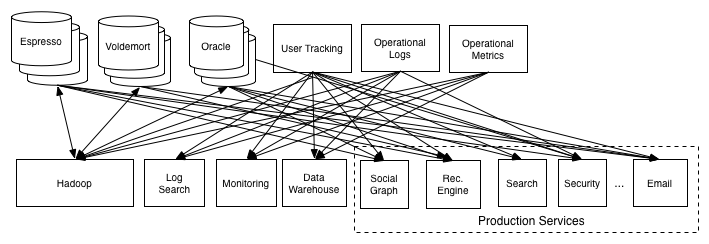
\includegraphics[width=1.0\textwidth]{images/datapipeline_complex.png}
    \caption{Complex Point-To-Point Architecture}
    \label{fig:datapipeline_complex}
\end{figure}

In this scenario several hurdles arise. The process of data integration would
have to be done for each system pair individually. At this point, an obvious
approach for a simplification would be to introduce an organization-wide
standardization of the data format. Thus, the integration process becomes 
significantly easier but still has to be done redundantly. Another problem that
remains are the tightly coupled systems. A simple change on one system could
affect one or more of it's connected systems directly, which is not only hard to
manage but also reduces the flexibility of further development of the landscape.
To extend the landscape the chances are high to touch existing systems which is
not only time intensive but also connected with risks regarding possible failures. In fact,
these are known issues of a Point-To-Point channel of traditional messaging and
is described in Section \ref{intro-messaging-pointtopoint}.

\subsection{Central Platform as Solution}
\label{intro-datastream-centralplatform}
A more elegant and reliable approach to solve the mentioned problems would be to
introduce a central platform, that is able to support both batch and real-time
consumption and thus is able to hold the described requirements given in table
\ref{table:requirements-batch-stream}. This system which can act as a single
data repository to isolated consumers and gives access to any data that is
required, as shown in figure \ref{fig:datapipeline_simple}. It aggregates
incoming events and represents an even stream for any its consumers. 

\begin{figure}[H]
    \centering
    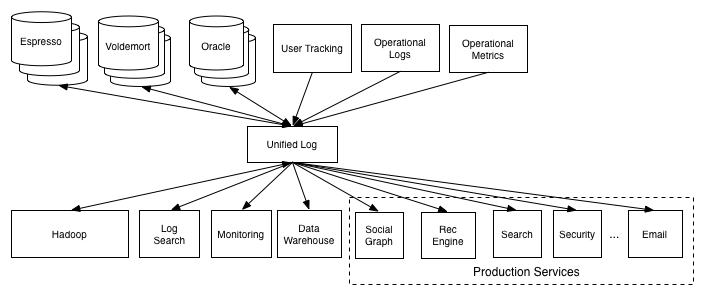
\includegraphics[width=1.0\textwidth]{images/datapipeline_simple.png}
    \caption{Broker Architecture}
    \label{fig:datapipeline_simple}
\end{figure}

In this constellation integrating a new data system---be it a data
source or a data destination---is fairly simple. Connecting it to a single
channel attached to the central platform is all what is needed to be done. Besides the
loosely coupled components, with this architecture it becomes possible to
centralize the process of data integration by doing so in a standardized way,
directly within the stream. Thus, a huge factor of complexity over the system
landscape is being reduced. In fact, this opens up a whole new set of
possibilities in organizational scalability. 

\newpage
\section{Link to Message Brokers}
As solution for a modern big data environment with huge amount of event data
which needs to be processed in different systems we need platform which acts as
mediator by handles the incoming event as stream and provide them to several
consumers (\ref{intro-datastream-centralplatform}). This seems to be very similar to
the definition of a message broker (\ref{intro-messaging-broker}) and indeed
these two concepts can be compared. Actually an event stream can be realised
with an underlying message broker and as we already described \todo{ref}, events
can be considered as messages with the event data as payload. In this point of
view the central stream platform is nothing else than a message broker which
handles incoming events, persist them in a queue and provide them for the
consumers which can be stream or batch processing systems. 
\begin{figure}[H]
    \centering
    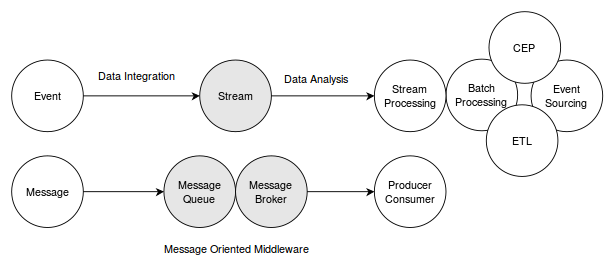
\includegraphics[width=0.8\textwidth]{images/messaging-vs-streaming.png}
    \caption{Event Stream vs Messaging}
    \label{fig:messaging-vs-streaming}
\end{figure}
Depending on the guarantees a message broker implementation provides the more it
is predestined for an event stream environment than others. In a survey (Chapter
\ref{survey-broker}) we examine the limits of traditional message brokers and
the needs for lately introduced systems such as Apache Kafka\cite{apachekafka},
Scribe\cite{scribe} or Flume\cite{apacheflume} and further try to compare and
categorize those systems after their strengths and weaknesses.

In the following Chapter \ref{intro-kafka} we examine capabilities for Apache
Kafka related to the functionalities of acting as a centralized event stream
platform. This gives not only a more concrete background of the components of a
state of the art message broker implementation but also serves as a basis for
the survey which is followed in Chapter \ref{survey-broker}.

%\section{Notes}

%-From traditional PCs and Smartphones to a lot of sensors who are connected to
%the interne -> Internet of Things!

%\todo[inline]{Einbringen des folgenden Statements: The nice thing about this
%architecture is that you can now have multiple consumers for the same event
%data. You can have one consumer which simply archives the raw events to some big
%storage; even if you don’t yet have the capability to process the raw events,
%you might as well store them, since storage is cheap and you can use them in
%future. Then you can have another consumer which does some aggregation (for
%example, incrementing counters), and another consumer which does something else.
%Those can all feed off the same event stream.}

\chapter{Apache Kafka}
\label{intro-kafka}

As this thesis is about the implementation of a message broker that correlates
to the functionalities Apache Kafka provide, we describe in the following the
components and functionalities of Apache Kafka in the current state (Version
0.8.2). This shall provide a basis for further comparison (see \ref{survey-broker}) with
more traditional broker systems, which is why won't provide any implementation
specific details in this section but describe the concepts in a higher level of
abstractness instead. Thus, it is also an overview and the initial position of our
own implementation (see \todo{ref}), in which Chapter the implementation
specific aspects will be resolved in detail. 

\section{Background}

Apache Kafka was initially developed at LinkedIn\cite{linkedin} and subsequently
released as an open source project with the Apache Software
Foundation\cite{apachefoundation}. 
\\ \\
Initially at LinkedIn the landscape was overwhelmed by the complexity due to
point-to-point (\ref{intro-messaging-pointtopoint})
pipelines that delivered data to a single destination with no
integration between. Messages were written to aggregated files and then copied
to ETL servers (data integration) and further loaded into data warehousing and batch
processing (\ref{intro-datastream-batchprocessing})
clusters. Thus, this service included the lack of real-time data access which
is---especially for a data driven company that populates activity-driven news
feeds---an essential requirement. In fact, this fragility and complexity of this
pipeline lead to inevitable delays in adding new types of activity data.
Besides the feature wise limitations, also the detection time of operational
problems increased over time due to the ever-increasing pressure on the latency
of the data warehouse processes. This could have been solved with
stream processing systems (\ref{intro-datastream-streamprocessing}) but again, 
due to the lack of any central platform (\ref{intro-datastream-centralplatform})
that can provide continuous data, was not supported at this point.
\cite{goodhope2012building}

\\ \\
First attempts towards a piece of infrastructure (e.g. broker) that can server
stream and batch processing systems were made by experimenting with
ActiveMQ\cite{activemq}. During tests under full production load they ran into
several significant problems. It turned out that if the queue backed up beyond what could
be kept in memory, performance would severely degrade due to heavy amounts of
random I/O. Inefficiencies had to be accepted regarding clustered consumers
requiring duplicating the data for each consumer in a separate queue. Further
difficulties were faced with ActiveMQ's built in persistence mechanism that lead
to very long restart times. 
\todo[inline]{well, reasons are not that overwhelming honestly...}
According to LinkedIn it would have been possible to provide enough buffer to
keep the ActiveMQ brokers above water but would have required hundred servers to
process a subset of activity data. As a result, the decision was made to build a
custom piece of messaging infrastructure targeting high-volume scale-out
deployment and thus serve batch and stream processing systems. 
\cite{goodhope2012building}


\section{Characteristics}
- Zitat: One key feature of Kafka is its functional simplicity. While there is a
lot of sophisticated engineering under the covers, Kafka’s general functionality
is relatively straightforward. Part of this simplicity comes from its
independence from any other applications (excepting Apache ZooKeeper)

\section{Use Cases}
\begin{description}
    \item [Traditional message broker]
    \item [Log aggregation]
    \item [Stream processing] Kafka's strong durability is very useful in the
        context of stream processing
\end{description}

\section{The Log}
\label{intro-kafka-log}
Apache Kafka uses a so-called commit log for managing messages within the
broker. This log has nothing in common with "application logging", as traces of
a software designed for human read. Instead, logs in the context of distributed systems
are designed for programmatic access. Basically it is a simple, append-only data
structure which contains a sequence of records ordered by time whereas each
entry is assigned to an unique number, called offset. Thanks to the strict
ordering insight a log the record offset can be used as timestamp whereas a log
gets decoupled from any time system. \cite{apachekafka} \cite{JK-TheLog}

\begin{figure}[H]
    \centering
    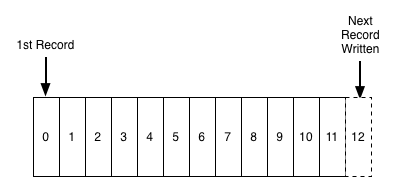
\includegraphics[width=0.4\textwidth]{images/log.png}
    \caption{The  Log \cite{JK-TheLog}}
    \label{fig:the-log}
\end{figure}

Apache Kafka handles a own log for every topic whereas the log contains all
published messages as single records. Compared to traditional messaging systems,
Kafka does not delete a record after consumption, actually it makes no difference
 whether or not they have been consumed. As we see later every consumer
controls its position of the log by its own. Instead Kafka holds record within a
defined window of data before it deletes the tail of the log. An additional
feature called log compaction can be activated to reduce the amount of messages
which need to be deleted by removing only obsolete records. \cite{apachekafka} \cite{JK-TheLog}

Facing the challenges of large distributed systems, a log must scale well. For
improving scalability and fault tolerance, Kafka can divide a log in multiple
partition. 

\begin{figure}[H]
    \centering
    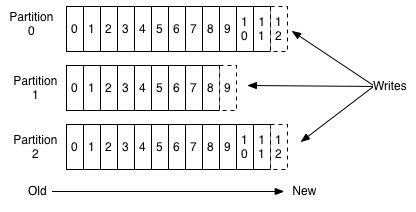
\includegraphics[width=0.5\textwidth]{images/log_anatomy.png}
    \caption{Partitioned Log \cite{apachekafka}}
    \label{fig:the-log}
\end{figure}

Logs originally come from databases where they are used to for replication
whereas the log includes records of what happened. Describing every replica by
the maximum log entry it has processed, the problem of coordinating
states of getting replicas is getting much easier. Apache Kafka uses this
approach for consumption of messages. Every consumer knows its actual offset and
advance it linearly as it reads messages from the log. The log can be seen as a
re-playable record of history whereas a consumer also can reset to an older
offset to reprocess. \cite{JK-TheLog}

\begin{figure}[H]
    \centering
    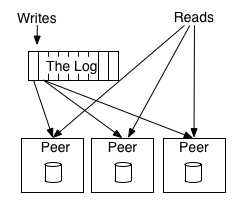
\includegraphics[width=0.4\textwidth]{images/state-machine-replication.png}
    \caption{Peers can sync their state with the log \cite{JK-TheLog}}
    \label{fig:the-log}
\end{figure}

\section{Components}
\subsection{Persistance}
Apache Kafka stores all data immediately to a persistent log
(\ref{intro-kafka-log}) 
and therefore relies heavily on the \gls{file system}.
Instead of flushing incoming messages from producers directly to the disks, the
data is stored as a compact byte structure within the \gls{page cache}.
\\ \\
The process of copying the data to the disk is handled by the operating system
that will not only use linear reads and writes \todo{gls} as a pattern for heavy
optimization but also provides read-ahead and write-behind techniques.
The latter will pre-fetch data in large block multiples and group smaller logical
writes into large physical writes. Thus, a SATA RAID-5 of six 7200rpm
disks will achieve a performance of 600MB/s in writes.
\\ \\
As a result of of the mentioned factors of using the file system and relying on
\gls{page cache} leads to the fact that Apache Kafka claims access to all free memory.
Doing so will result in a cache of up to 28-30GB on a 32GB machine. In a default
setup, data is kept in memory for 7 days to provide data required for processing
directly from the memory. This duration should be set according to of one's own
needs. In fact, the memory stays persistent during a restart of the Kafka
service but won't if the server restarts for example. In the latter scenario,
Apache Kafka will restore all data from the disk to the memory.
\\ \\
One drawback following this model of not immediately writing data to disk can not be
omitted. A small number of messages can be lost in the event of a hard server
failure before messages are transfered to the Kafka brokers or flushed to disk. 

\subsection{Message Delivery}
\label{kafka-message-delivery}
\todo[inline]{kafka = pull based model}
\todo[inline]{kafa's guarantees regarding message delivery}
\subsection{Replication}
To hold the defined guarantees (\ref{kafka-message-delivery}) regarding to system
or network failures, Apache Kafka supports \gls{replication} on the level of log
partitions \todo{ref}. Thereby it can replicate specific topics across a configurable
number of other other Kafka nodes. Every topic has a defined leader node which
is active in normal operation. A leader node can have zero or more followers
which are responsible for replicating the entries of the leader log. The followers
do this by simply act as a normal Kafka consumer of the leader node and
constantly update their own log so that it is identical. Every incoming message
needs to be replicated by every follower node before any other consumer can get
it. A fully replicated message is considered as "commited". This guarantees that
the consumer need not worry about potentially seeing a message that could be
lost if the leader fails. \cite{apachekafka}

\todo[inline]{illustration}


\todo[inline]{zookeeper}

\subsection{Compression}

\subsection{Batching}

%\subsection{The Producer}

%\subsection{The Consumer}
%While many brokered message queue systems have the broker maintain the state of
%its consumers, Kafka does not.

\subsubsection{Grouping}

\subsubsection{Ordering (offset)}

\section{Configuration Management (Zookeeper)}
\subsection{PAXO Algorithm}


\part{Technical Report}
\chapter{Specification}
\section{Purpose}
The prestudy of this thesis gives an insight in the fundamentals of messaging, especially
the purpose of message brokers for big data event streaming. We also compare
the most related broker implementations and provide detailed information about Apache
Kafka. The second part of this work is focusing on the implementation of a message
broker in the functional program language Haskell\todo{ref}. The goal is to get
use of the advantages of the functional paradigm regarding to the resulting
throughput performance. By using the example of Apache Kafka the main purpose
lies on building a server application which implements the main functionality of
Apache Kafka. 

\section{Features}
\begin{table}[h]
\begin{tabular}{lll}
\textbf{Functionality}       & \textbf{Description} & \textbf{Part of Thesis} \\
Server Implementation        &                      & yes                     \\
Wire Protocol Implementation &                      & yes                     \\
API for Haskell Clients      &                      & yes                     \\
Thin Haskell Clients         &                      & yes                     \\
Producing Messages           &                      & yes                     \\
Consuming Messages           &                      & yes                     \\
Log Persistency              &                      & yes                     \\
Error Handling               &                      & yes                     \\
Message Batching             &                      & yes                     \\
Message Compression          &                      & no                      \\
Partitioning                 &                      & partly                  \\
Log Compaction               &                      & no                      \\
Broker Replication           &                      & no                      \\
Broker Recovery              &                      & no                      \\
Consumer Groups              &                      & no                      \\
Zookeeper Integration        &                      & no                     
\end{tabular}
\end{table}

\section{Components}

Basically, the architecture consists of two main components namely the broker and
the client, whereas the client can act as producer, consumer or both. The broker
is a server which only reacts to requests that are sent from clients. Every
request contains an API key which the broker uses to determine which action it
has to do (e.g. persist produced message or consume message). For each valid
request the broker sends back a corresponding response to the client which
either includes the fetched data or an error code. The broker never communicates
with a client without a request.

\begin{figure}[H]
    \centering
     \begin{sequencediagram}
        %\newthread{broker}{Broker}
         \newinst[3]{client}{Client}
         \newinst[3]{broker}{Broker}
        \begin{messcall}
            {client}{(1) Send Request}{broker}{}
        \end{messcall}
        \begin{messcall}
            {broker}{(2) Do Action}{broker}{}
        \end{messcall}
        \begin{messcall}
            {broker}{(3) Send Response}{client}{} 
        \end{messcall}
     \end{sequencediagram}
     \caption{Basic communication between client (producer or consumer) and
     broker}
\end{figure}

\section{Workflow}

The main purpose of this broker implementation can be split in two cases. Case
one covers producing a message and persisting in the brokers log. Case two
allows to consume persisted messages on request. As for clients, depending on
which API to be used, the client can act either as producer or consumer.

\subsection{Produce messages}

In the case of a producer client, the following workflow highlights the
fundamental steps being passed from sending a request by the client to
persisting the message on the broker.

\begin{figure}[H]
    \centering
    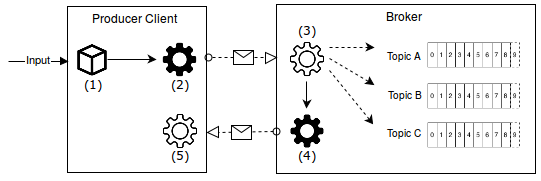
\includegraphics[width=0.8\textwidth]{images/concept_producer.png}
    \caption{Case one: Producer Workflow}
    \label{fig:conept-producer}
\end{figure}

\begin{description}
    \item [(1)] 
        {Packing Produce Request: Getting input data to protocol conform data structure.}
    \item [(2)] 
        {Serializing and send Produdce Request: Encoding data structure to an
            binary  string and transmit over a tcp socket to the broker.}
    \item [(3)] 
        {Parsing and Handling Produce Request: Broker receives the binary string
            and parse it back to the appropriate data structure. The request
            handler of the  broker checks the API Key of the request. If it is a
            produce request, the containg message will be written to the
            appropriate topic log.}
    \item [(4)] 
        {Send Produce Response: A response is packed, serialized and transmitted
            back to the client. The response contains an error code which has
            the value 0 if everything worked well otherwise another value for a
            specific problem. }
    \item [(5)] 
        {Parse Produce Response: Producer client receives a binary string and
            parses it to valid response data structure }
\end{description}

\subsection{Consume messages}

The case where the client acts as a consumer, the workflow does not distinguish from
producing message. Instead of the translation from request message to the log, persisted messages
are read from the log and are delivered from the broker to the client.

\begin{figure}[H]
    \centering
   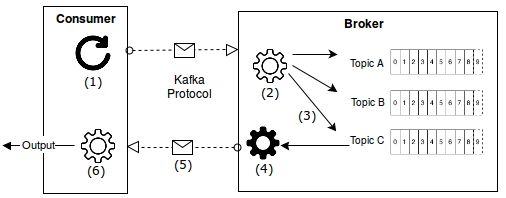
\includegraphics[width=0.7\textwidth]{images/concept_consumer.png}
    \caption{Case two: Consumer Workflow}
    \label{fig:concept-consumer}
\end{figure}

\begin{description}
    \item [(1)] 
        {Continously send fetch request: Consumer client sends fetch
        requests in configurable intervall as binary string to the broker. } 
    \item [(2)] 
        {Parsing and handling fetch request: Broker receives the binary string
            and parse it back to the appropriate data structure. The request
            handler of the broker checks the API Key of the request. If it is a
            fetch request, the broker reads messages of the requested topic and
            packs it to a fetch response. message will be written to the
            appropriate topic log.}
    \item [(3)] 
        {Send fetch response: The fetch request which contains the requested
        messages is send back to the consumer client.}
    \item [(4)] 
        {Parse Response:Consumer client receives a binary string and parses it
        to valid response data structure }
\end{description}


%\chapter{Architecture}


\section{Design decisions}
\subsection{Protocol}
For communicating over network we implement a binary protocol based on tcp.
Because we use Apache Kafka as benchmark for this project and we want to provide
compatibility to existing Kafka clients, we decided to fully implement the Kafka
Protocol version 0.8.x \todo{ref}. It differ in six APIs which each of it is
defined with a request-response message pair. The client initiates a socket connection and then
writes a sequence of request messages and reads back the corresponding response
message. 

TODO: What design desicions we made regarding the protocol? (Types, Serializer,
Parser). 

\subsection{Separation} 
\label{sec:separation}
Both, the client and broker component need to use the same underlying protocol for
communication. Therefore we provide a third component which fully implements the Apache Kafka
protocol \todo{ref} and provides the appropriate functions and types as library.
This component fully separates the clients from the broker. It also allows to
use the clients with other Kafka based broker implementations, especially Apache
Kafka itself. 

To support interoperability we want to simplify the implementation of a broker
client. Therefore we provide a client library which provides functionalities to
easily implement a Haskell client. The goal of this, is to be able to
setup a client without knowing too much details about the Apache Kafka protocol
itself. We therefore provide separate types to construct a message very easily.
In the background we then pack the input to the appropriate Request/Response
Message. 

\begin{figure}[H]
    \centering
    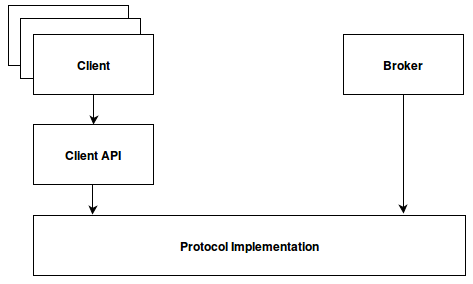
\includegraphics[width=0.55\textwidth]{images/architecture-components.png}
    \caption{Separation of code}
    \label{fig:architecture-components.png}
\end{figure}

\subsection{Consumption Model}
TODO: All requests are initiated by the client, and result in a corresponding
response message from the server





\chapter{Implementation Protocol}
\label{sec-protocol}
First of all we started to implement the Kafka protocol \todo{ref}
as data basis for all further functionality. The definition of the original
protocol is given as context free grammar for the request and response binary
format. Therefore it seemed likely to adopt the rules of the grammar to our
protocol implementation by map them with the Haskell type system. In a second
step we implemented encoder and decoder functions for getting messages from data
structure to binary format and backwards. As decided in \ref{sec:separation}, we
also provide a client library to isolate client implementations from details
about the protocol. 

Therefore our protocol implementation consists of the following modules: 
\begin{itemize}
    \item {Types: Mapping the protocol definition with Haskell type system. }
    \item {Decode: Provide functions to parse binary data to valid structure. }
    \item {Encode: Provide functions to serialize a given structure to a binary
        format. }
    \item {Client: Provide functions to simplify a Haskell client.}
\end{itemize}


A complete implementation of the Apache Kafka Protocol would
go beyond the scope of this thesis as the focus lies not
only in implementing the protocol but also to provide broker
functionality (see Chapter \ref{chap:broker}). Thus, most important is
the ability to produce and fetch messages. The following list gives 
an overview of what part of the protocol is implemented and what remains open:

\begin{itemize}
    \item Metadata API
    \begin{itemize}
        \tick Topic Metadata Request
        \tick Metadata Response
    \end{itemize}
    \item Produce API
    \begin{itemize}
        \tick Produce Request
        \tick Produce Response
    \end{itemize}
    \item Fetch API
    \begin{itemize}
        \tick Fetch Request
        \tick Fetch Response
    \end{itemize}
    \item Offset API
    \begin{itemize}
        \fail Offset Request
        \fail Offset Response
    \end{itemize}

    \item Offset Commit/Fetch API
    \begin{itemize}
        \fail Consumer Metadata Request
        \fail Consumer Metadata Response
        \fail Offset Commit Request
        \fail Offset Commit Response
        \fail Offset Fetch Request
        \fail Offset Fetch Response
    \end{itemize}
\end{itemize}

\section{Types}
The design of the Apache Kafka protocol allows to make a distinction between three kind of types:
\begin{enumerate}
  \item Related to request
  \item Related to response
  \item Related to data (for either request or response but can also be used for the \fnurl{Apache Kafka Log}{http://kafka.apache.org/documentation.html\#log} component since log files (on-disk) hold the same structure)
\end{enumerate}

As mentioned before, the representation of the protocol structure is implemented using the Haskell \fnurl{type
system}{https://wiki.haskell.org/Type}, more concrete using data types created
for our need using the named fields - also known as \fnurl{record
syntax}{http://en.wikibooks.org/wiki/Haskell/More_on_datatypes}. Given this, a
further step of abstraction is introduced by creating types for the binary
representation of a protocol field. 

\subsection{Naming convention}
As for request and response related types we had to introduce an own naming
convention. As a matter of fact, not every field of some kind of request or
response will be unique. For more than once, there is a field that will
represent a \textit{topicName} for example. Thus, naming the field \textit{
topicName} would have been the obvious solution but since the record syntax in
Haskell won't allow to use the same name for a field twice - even in different
data types - we defined unique prefixes for each request and response as being
listed in the following table:

\begin{table}[H]
\centering
\begin{tabular}{|l|l|l|}
\hline
\textbf{API}            & \textbf{Request (Rq)} & \textbf{Response (Rs)} \\ \hline
Metadata API (Md)       & MetadataRequest       & MetadataResponse       \\ \hline
Produce API (Pr)        & ProduceRequest        & ProduceResponse        \\ \hline
Fetch API (Ft)          & FetchRequest          & FetchResponse          \\ \hline
Offset API (Of)         & OffsetRequest         & OffsetResponse         \\ \hline
Offset Commit API (Ofc) & OffsetCommitRequest   & OffsetCommitResponse   \\ \hline
Offset Fetch API (Oft)  & OffsetFetchRequest    & OffsetFetchResponse    \\ \hline
\end{tabular}
\end{table}

%\subsubsection{Example}
As a result, a typical data type is described as follows, while details are
hidden for demonstration purposes.:

\begin{lstlisting}
-- more
data Partition =
    ----------------------
    -- ProduceRequest (pr)
    ----------------------
    RqPrPartition
    { rqPrPartitionNumber :: !PartitionNumber
    , rqPrMessageSetSize  :: !MessageSetSize
    , rqPrMessageSet      :: [MessageSet]
    }
    |
    ----------------------
    -- FetchRequest (ft)
    ----------------------
    RqFtPartition
    { rqFtPartitionNumber :: !PartitionNumber
    , rqFtFetchOffset     :: !Offset
    , rqFtMaxBytes        :: !MaxBytes
    }
    |
-- more
\end{lstlisting}


\subsection{Batching}
\label{impl-prot-batching}
A significant characteristic of the Kafka protocol is the ability to optimize
efficiency due to the batching of multiple message in one single request. Both
the API to send messages and the API to consume messages always work with a
sequence of messages and not only a single message. It is also possible to batch
messages across multiple topics and partitions. It is task of the client
implementation to use this ability clever but it also can ignore it and sends everything
one at a time. Batching leads to sequences of the same type in one request or response. Within
the protocol format this is defined by an array type. In our protocol
implementation the batching sequences are implemented with Haskell lists which
contains N repetitions of another type. Sequences can also be nested. 

As example, the following grammar rule of the original definition shows the
support of batching in the protocol. A batching sequence of a structure A is
shown as [A]:
\begin{lstlisting}
ProduceRequest => 
    RequiredAcks Timeout [TopicName [Partition MessageSetSize MessageSet]]
\end{lstlisting}

\subsection{Primitive Types}

The actual type for the data fields in the protocol have to match an unsigned
integer type of its length. This can easily be done using the
\fnurl{Data.Word}{http://hackage.haskell.org/package/base-4.7.0.2/docs/Data-Word.html}
library. However, while repetitive writing \textit{WordX} (where is stands for
8-, 16-, 32-, or 64 bit) is rather intuitive, creating aliases using the
\textit{type} keyword will result in better readable code, as well as structure
of the implemented protocol. 

%Sumarized, all protocol related types are size delimited and
%are made up of the following primitive types: 
\begin{table}[H]
    \begin{tabular}{| p{3cm}| p{7cm} | p{5cm} |}
\hline
\textbf{Type} & \textbf{Description} & \textbf{Used Haskell Library} \\ \hline
Fixed Width Primitives     & Signed integers stored in big endian order.
& Data.Word8, Word16, Word32, Word64 \\ \hline
Variable Length Primitives & Consist of a signed integer giving a length N
followed by N bytes of content. A length of -1 indicates null. String uses an
int16 (Data.Word16) for its size, and bytes uses an int32 (Data.Word32).    &
Data.ByteString(.Lazy) \\ \hline
Arrays                     & Repeated structures. Always be encoded as an int32
size containing the length N followed by N,repetitions of the structure which
can itself be made up of other,primitive types & Data.List                          \\ \hline
\end{tabular}
\end{table}

\subsection{Error Codes}
\label{subsec:protocol-types-error-codes}

To handle errors, the protocol specifies error codes they can be sent within a
response message. To adapt those codes, a data type \lstinline{ErrorCode}
deriving from
\fnurl{\lstinline{Enum}}{http://hackage.haskell.org/package/base-4.8.0.0/docs/Prelude.html\#t:Enum} is provided and implicitly represents the
appropriate error code by its order.

\begin{code}
data ErrorCode =
        NoError
      | Unknown
      | OffsetOutOfRange
      | InvalidMessage
      | UnknownTopicOrPartition
      | InvalidMessageSize
      | LeaderNotAvailable
      | NotLeaderForPartition
      | RequestTimedOut
      | BrokerNotAvailable
      | ReplicaNotAvailable
      | MessageSizeTooLarge
      | StaleControllerEpochCode
      | OffsetMetadataTooLargeCode
      | OffsetsLoadInProgressCode
      | ConsumerCoordinatorNotAvailableCode
      | NotCoordinatorForConsumerCodeA
        deriving (Show, Enum)
\end{code}

\subsection{Types related to Request}
A request message is the on-wire format of data which is getting from client to
broker.

Each request message has its same header fields independent for which API they are used. 
The real payload of the request is individual to the particular API which is
used. 

\begin{figure}[H]
    \centering
    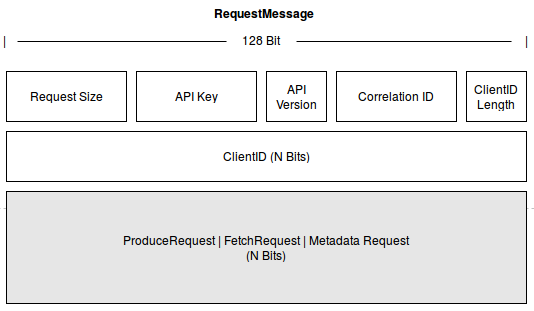
\includegraphics[width=0.7\textwidth]{images/impl-prot-types-requestMessage.png}
    \caption{Format of type RequestMessage}
    \label{fig:impl-prot-types-requestMessage}
\end{figure}

\begin{table}[H]
\centering
\begin{tabular}{ l  l  p{10cm} }
\hline
RequestSize   & Data.Word16     & Gives the size of the subsequent request message in bytes. The client can read requests by first reading this 4 byte size as an integer N and then reading and parsing the subsequent N bytes of the request. \\ \hline
ApiKey        & Data.Word32     & This is a numeric id for the API being invoked                                                                                                                                                              \\ \hline
ApiVersion    & Data.Word32     & Number of element in following list.                                                                                                                                                                          \\ \hline
CorrelationId & Data.Word32     & Will be passed back in the response by the broker unmodified. It is useful for matching request and response between the client and server.                                                                   \\ \hline
StringLength  & Data.Word16     & Length, in bytes, of string ClientId                                                                                                                                                                          \\ \hline
ClientID      & Data.ByteString & Identifier for the client application                                                                                                                                                                         \\ \hline
Request       &                 & API specific Request type (either ProduceRequest, FetchRequest, or others)                                                                                                                                    \\ \hline
\end{tabular}
\end{table}

TODO: Because the RequestSize is only needed once to determine the length of the whole Request, it is is not part of the type RequestMessage

\subsubsection{ProduceRequest}
Request Payload for Produce API. Sends MessageSet's (see 
\ref{impl-protocol-types-data}) to the broker. For efficiency it allows sending
message sets intended for many topic partitions in a single request (see
\ref{impl-prot-batching}). MessageSets are not preceded by an int32 like other
array elements in the protocol.

\begin{figure}[H]
    \centering
    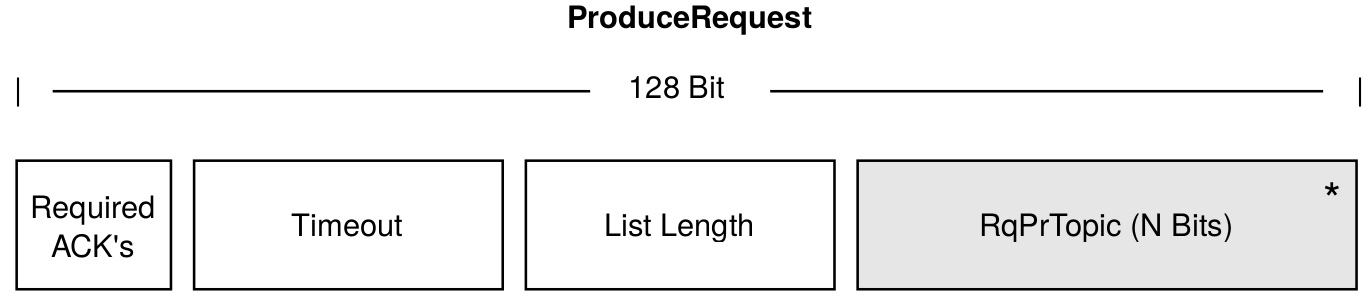
\includegraphics[width=0.7\textwidth]{images/impl-prot-types-produceRequest.png}
    \caption{Format of type ProduceRequest; * = N repetitions }
    \label{fig:impl-prot-types-produceRequest}
\end{figure}

\begin{table}[H]
\centering
\begin{tabular}{ l  l  p{10cm} }
\hline
RequiredAcks  & Data.Word16 & This field indicates how many acknowledgements the broker should receive before responding to the request.                       \\ \hline
Timeout       & Data.Word32 & This provides a maximum time in milliseconds the broker can await the receipt of the number of acknowledgements in RequiredAcks. \\ \hline
ListLength    & Data.Word32 & Number of element in following list.                                                                                             \\ \hline
{[}RqPrTopic{]} & Data.List   & Sequence of RqPrTopics, see below.                                                                                                  \\ \hline
\end{tabular}
\end{table}

TODO: Functionality of ReqAcks and Timeout are not implemented yet. 

A ProduceRequest includes N repetitions of the RqPrTopic type whereas the producer
client is able to send messages for multiple different topics:

\begin{figure}[H]
    \centering
    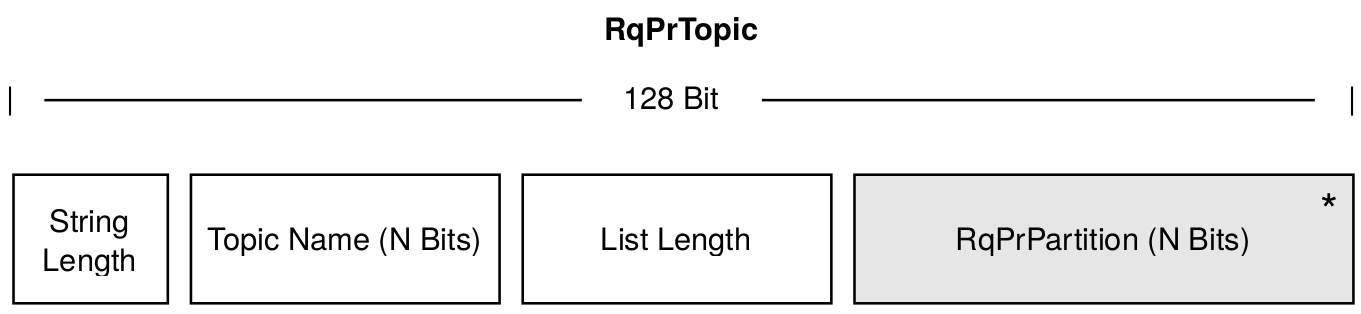
\includegraphics[width=0.7\textwidth]{images/impl-prot-types-prTopic.png}
    \caption{Format of type RqPrTopic; * = N repetitions }
    \label{fig:impl-prot-types-produceRequest}
\end{figure}

\begin{table}[H]
\centering
\begin{tabular}{ l  l  p{10cm} }
\hline
StringLength      & Data.Word16     & Length, in bytes, of string TopicName.              \\ \hline
TopicName         & Data.ByteString & Name of the topic that data is being published to. \\ \hline
ListLength        & Data.Word32     & Number of element in following list.                \\ \hline
[RqPrPartition] & Data.List          & Sequence of PrPartitions, see below.                \\ \hline
\end{tabular}
\end{table}

The RqPrTopic in turn includes N repetitions of the RqPrPartition type
whereas the producer client is able to send message for multiple partitions
within a topic.  

\begin{figure}[H]
    \centering
    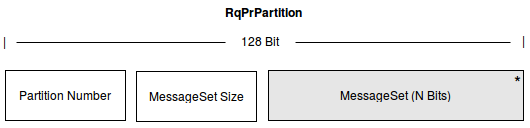
\includegraphics[width=0.7\textwidth]{images/impl-prot-types-prPartition.png}
    \caption{Format of type RqPrTopic; * = N repetitions }
    \label{fig:impl-prot-types-produceRequest}
\end{figure}

\begin{table}[H]
\centering
\begin{tabular}{ l  l  p{11cm} }
\hline
PartitionNumber & Data.Word32 & The partition Id that data is being published to.                                                                                                                                        \\ \hline
MessageSetSize  & Data.Word32 & Sequences of MessageSet's are not preceded by an int32 like other array elements in the protocol. Instead, this field determines the total size, in bytes, of the following MessageSet's. \\ \hline
[MessageSet]      & Data.List      & Finally the RqPrPartition type also holds the actual messages (as defined in \ref{impl-protocol-types-data}.                                                                                \\ \hline
\end{tabular}
\end{table}

\subsubsection{FetchRequest}
Request Payload for Fetch API. Fetchs chunk of one or more logs for some
topic-partitions. Defines a starting offset at which to begin fetch. 

\begin{figure}[H]
    \centering
    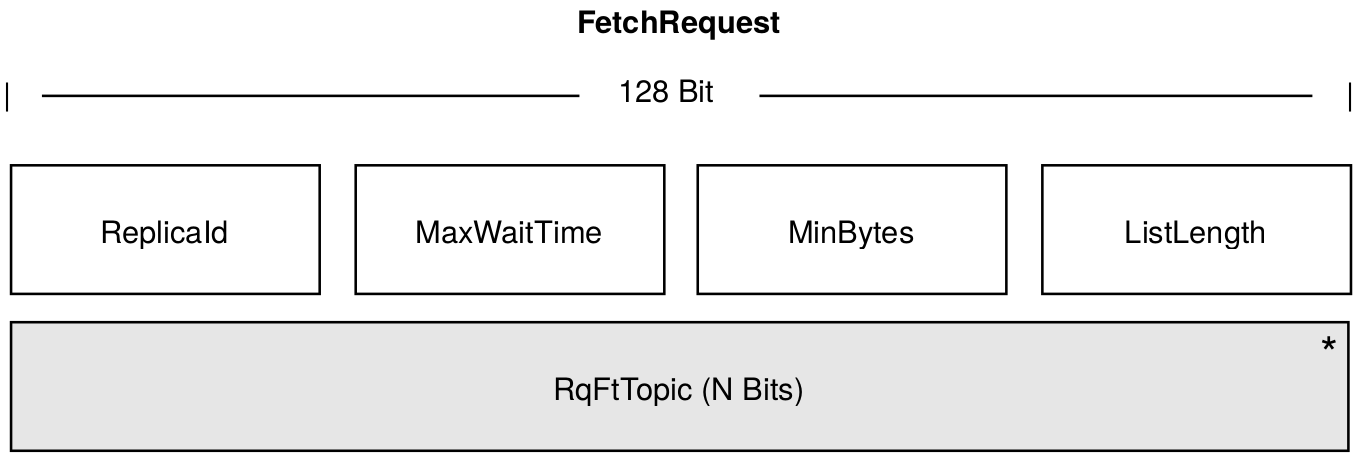
\includegraphics[width=0.7\textwidth]{images/impl-prot-types-fetchRequest.png}
    \caption{Format of type FetchRequest; * = N repetitions }
    \label{fig:impl-prot-types-fetchRequest}
\end{figure}

\begin{table}[H]
\centering
\begin{tabular}{ l  l  p{11cm} }
\hline
ReplicaId      & Data.Word32 & Indicates the node id of the replica initiating this request. (Not yet used in broker implementation)                        \\ \hline
MaxWaitTime    & Data.Word32 & Maximum amount of time in milliseconds to block,waiting if insufficient data is available at the time the request is,issued. \\ \hline
MinBytes       & Data.Word32 & Minimum number of bytes of messages that must be available to give a response.                                               \\ \hline
ListLength     & Data.Word32 & Number of elements in following list.                                                                                        \\ \hline
{[}FtTopics{]} & Data.List   & Sequence of FtTopics, see below                                                                                              \\ \hline
\end{tabular}
\end{table}

\begin{figure}[H]
    \centering
    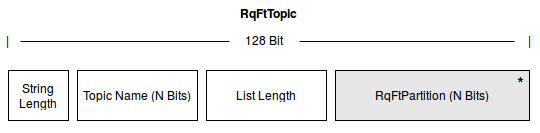
\includegraphics[width=0.7\textwidth]{images/impl-prot-types-ftTopic.png}
    \caption{Format of type RqFtTopic; * = N repetitions }
    \label{fig:impl-prot-types-ftTopic}
\end{figure}

\begin{table}[H]
\centering
\begin{tabular}{ l  l  p{10cm} }
\hline
StringLength      & Data.Word16     & Length, in bytes, of string TopicName.              \\ \hline
TopicName         & Data.ByteString & Name of the topic the fetch is for . \\ \hline
ListLength        & Data.Word32     & Number of element in following list.                \\ \hline
[FtPartition]     & Data.List       & Sequence of FtPartitions, see below.                \\ \hline
\end{tabular}
\end{table}

\begin{figure}[H]
    \centering
    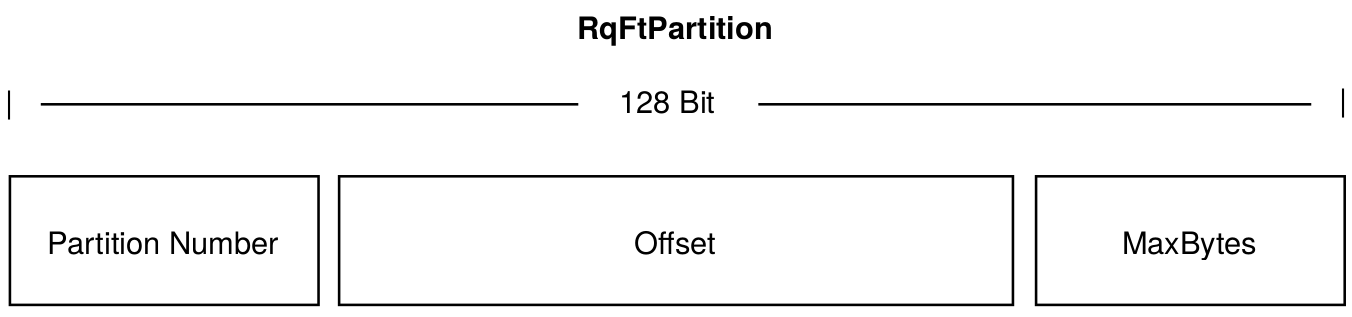
\includegraphics[width=0.7\textwidth]{images/impl-prot-types-ftPartition.png}
    \caption{Format of type RqFtPartition }
    \label{fig:impl-prot-types-ftPartition}
\end{figure}

\begin{table}[H]
\centering
\begin{tabular}{ l  l  p{10cm} }
\hline
PartitionNumber & Data.Word32 & Id of the partition the fetch is for.                                          \\ \hline
Offset          & Data.Word64 & Offset to begin the fetch from.                                                \\ \hline
MaxBytes        & Data.Word32 & Minimum number of bytes of messages that must be available to give a response. \\ \hline
\end{tabular}
\end{table}

\subsection{Types related to Response}
A response message is the on-wire format of data which is getting from broker to
client.

Each request message has its same header fields independent for which API they are used. 
The real payload of the request is individual to the particular API which is
used. A response will always match the paired request (e.g. a ProduceResponse is
sent in return to a ProduceRequest).

\begin{figure}[H]
    \centering
    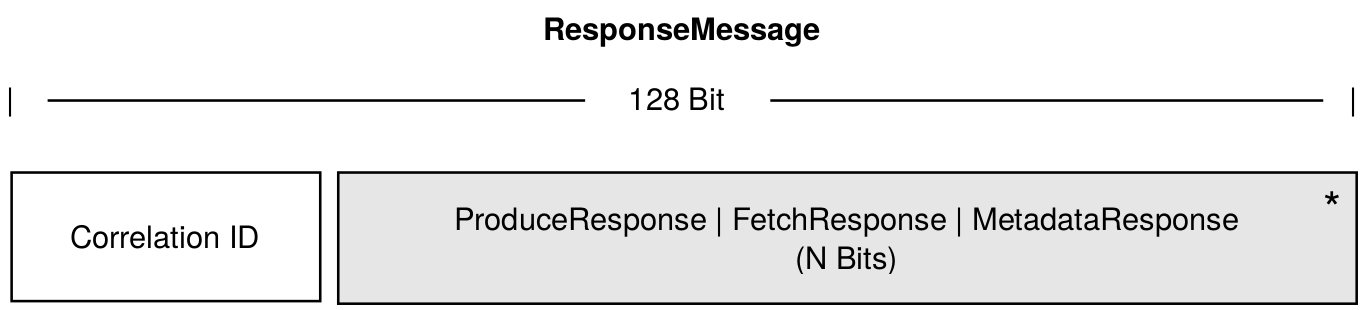
\includegraphics[width=0.7\textwidth]{images/impl-prot-types-responseMessage.png}
    \caption{Format of type ResponseMessage; * = N repetitions}
    \label{fig:impl-prot-types-responseMessage}
\end{figure}

\begin{table}[H]
\centering
\begin{tabular}{ l  l  p{10cm} }
\hline
CorrelationId  & Data.Word32 & Id that is supplied by request is passed back
(for request-reply reference).              \\ \hline
{[}Response{]} & Data.List   & Sequence of Responses of the same type (either
ProduceResponse, FetchResponse or others). \\ \hline
\end{tabular}
\end{table}


\subsubsection{ProduceResponse}
Response Payload for Produce API. Sends an ErrorCode which determines whether a
produce request for e specific topic-partition succeeded (ErrorCode 0 ) or ended
in a particular failure. 

\begin{figure}[H]
    \centering
    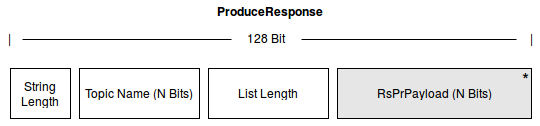
\includegraphics[width=0.7\textwidth]{images/impl-prot-types-produceResponse.png}
    \caption{Format of type ProduceResponse; * = N repetitions}
    \label{fig:impl-prot-types-produceResponse}
\end{figure}

\begin{table}[H]
\centering
\begin{tabular}{ l  l  p{10cm} }
\hline
StringLength      & Data.Word32     & Length, in bytes, of string TopicName. \\ \hline
TopicName         & Data.ByteString & Name of the topic this response entry corresponds to.\\ \hline
ListLength        & Data.Word32     & Number of element in following list.\\ \hline
{[}RsPrPayload{]} & Data.List       & Sequence of RsPrPayload, see below.
\\ \hline
\end{tabular}
\end{table}

\begin{figure}[H]
    \centering
    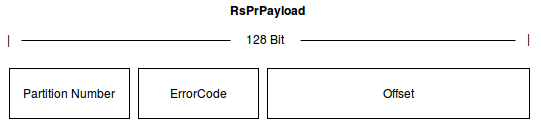
\includegraphics[width=0.7\textwidth]{images/impl-prot-types-prPayload.png}
    \caption{Format of type RsPrPayload. * = N repetitions}
    \label{fig:impl-prot-types-prPayload}
\end{figure}


\begin{table}[H]
\centering
\begin{tabular}{ l  l  p{10cm} }
\hline
PartitionNumber & Data.Word32 & Number of partition this response entry
corresponds to.                                                \\ \hline
ErrorCode       & Data.Word16 & Topic-Partition specific error code. Error code
0 determines that data has been published successfully. \\ \hline
Offset          & Data.Word64 & Number of element in following list.
\\ \hline
\end{tabular}
\end{table}

\subsubsection{FetchResponse}
Response Payload for Fetch API. Sends requested chunk of one ore more logs as
sequence of MessageSet's (see \ref{impl-protocol-types-data}). 

\begin{figure}[H]
    \centering
    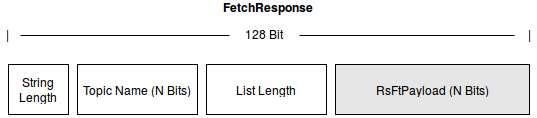
\includegraphics[width=0.7\textwidth]{images/impl-prot-types-fetchResponse.png}
    \caption{Format of type FetchResponse}
    \label{fig:impl-prot-types-fetchResponse}
\end{figure}

\begin{table}[H]
\centering
\begin{tabular}{ l  l  p{10cm} }
\hline
StringLength      & Data.Word32     & Length, in bytes, of string TopicName. \\ \hline
TopicName         & Data.ByteString & Name of the topic this response entry corresponds to.\\ \hline
ListLength        & Data.Word32     & Number of element in following list.\\ \hline
{[}RsPrPayload{]} & Data.List       & Sequence of RsPrPayload, see below.
\\ \hline
\end{tabular}
\end{table}

\begin{figure}[H]
    \centering
    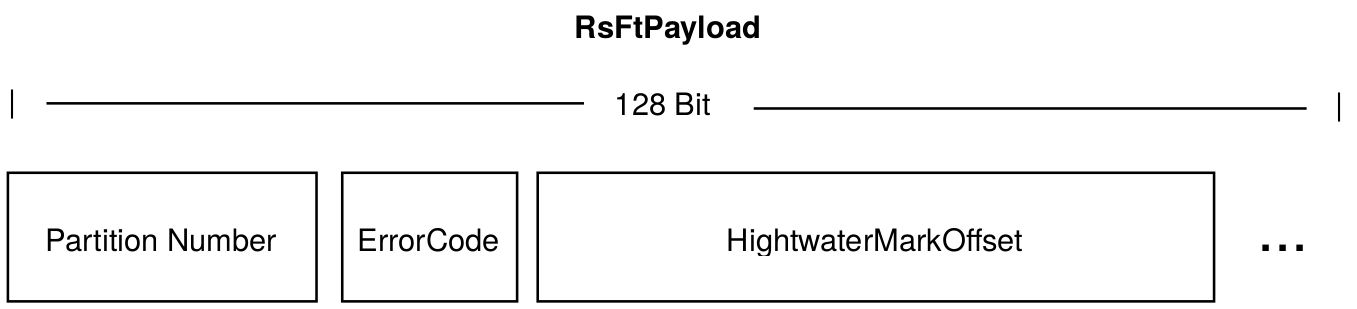
\includegraphics[width=0.7\textwidth]{images/impl-prot-types-ftPayload.png}
    \caption{Format of type RsFtPayload}
    \label{fig:impl-prot-types-ftPayload}
\end{figure}

\begin{table}[H]
\centering
\begin{tabular}{ l  l  p{10cm} }
\hline
PartitionNumber     & Data.Word32 & Number of partition this response entry corresponds to.                                                                                               \\ \hline
ErrorCode           & Data.Word16 & Topic-Partition specific error code. Error code 0 determines that data has been published successfully                                                \\ \hline
HighwaterMarkOffset & Data.Word64 & The offset at the end of the log for this partition. This can be used by,the client to determine how many messages behind the end of the log,they are \\ \hline
MessageSetSize      & Data.Word32 & The size in bytes of the message set for this topic-partition                                                                                         \\ \hline
{[}MessageSet{]}    & Data.List   & The message data fetched from this partition, in the format described below                                                                           \\ \hline
\end{tabular}
\end{table}

\subsection{Types related to Data}
\label{impl-protocol-types-data}
The actual transported data has a common structure,
called a MessageSet. This format happens to be used both for the on-disk storage on the
broker and the on-the-wire format. Therefore the broker do not need to perform
any transformations to the actual message when persisting to the log or read
from it. 

\begin{figure}[H]
    \centering
    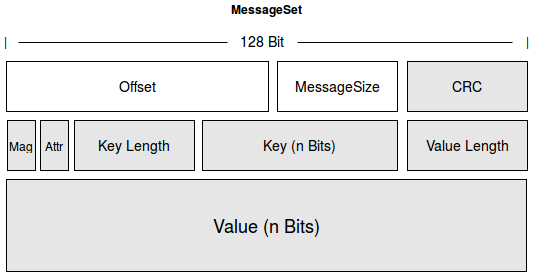
\includegraphics[width=0.7\textwidth]{images/impl-prot-types-messageSet.png}
    \caption{Format of type MessageSet}
    \label{fig:impl-prot-types-messageSet}
\end{figure}

\begin{table}[H]
\centering
\begin{tabular}{ l  l  p{11cm} }
\hline
Offset      & Data.Word64 & Determines log offset number in log.  When the producer is sending messages it doesn't actually know the offset and can fill in any value here it likes. \\ \hline
MessageSize & Data.Word32 & Determines size of Message in Bytes.               \\ \hline
Message     &     & Message format, see below.                                                                                                                    \\ \hline
\end{tabular}
\end{table}

\subsubsection{Message}
Message is part of the MessageSet and contains a checksum to check integrity of
the actual payload of the message. To abstract the fields which are checked we
combine them in another type, see Payload.

\begin{figure}[H]
    \centering
    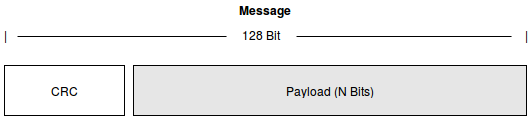
\includegraphics[width=0.7\textwidth]{images/impl-prot-types-message.png}
    \caption{Format of type Message}
    \label{fig:impl-prot-types-message}
\end{figure}

\begin{table}[H]
\centering
\begin{tabular}{ l  l  p{11cm} }
\hline
CRC     & Data.Word32 & The CRC is the CRC32 of the remainder of the message bytes. This is used,to check the integrity of the message on the broker and consumer. \\ \hline
Payload &      & Payload format, see below.                                                                                                                  \\ \hline
\end{tabular}
\end{table}

\subsubsection{Payload}
This types defines the actual payload of a message with its meta info.

\begin{figure}[H]
    \centering
    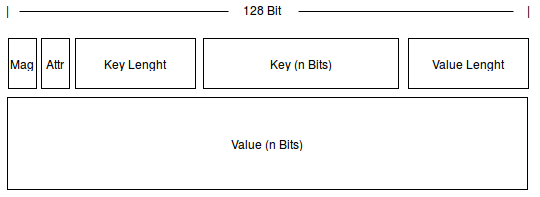
\includegraphics[width=0.7\textwidth]{images/impl-prot-types-payload.png}
    \caption{Format of type Payload}
    \label{fig:impl-prot-types-payload}
\end{figure}

\begin{table}[H]
\centering
\begin{tabular}{ l  l  p{10cm} }
\hline
Magic       & Data.Word8      & This is a version id used to allow backwards compatible evolution of the message binary format. The current value is 0.                                         \\ \hline
Attributes  & Data.Word8      & This byte holds metadata attributes about the message. The lowest 2 bits,contain the compression codec used for the message. The other bits,should be set to 0. \\ \hline
KeyLen      & Data.Word32     & Determines length of Key field in bytes.                                                                                                                         \\ \hline
Key         & Data.ByteString & The key is an optional message key that is used for partition assignment. The key can be null.                                                                  \\ \hline
ValueLength & Data.Word32     & Determines length of Value field in bytes.                                                                                                                      \\ \hline
Value       & Data.ByteString & The actual message contents as an opaque byte array. The message can be null.                                                                                   \\ \hline
\end{tabular}
\end{table}

TODO: Kafka supports recursive messages in which case this may itself contain a message set. --> not implemented yet  

%\subsection{API's}
%\todo{-> verschieben in Kap Kafka detail? }
%\subsubsection{Metadata API}
%Describes the currently available brokers, their host and port information, and
%gives information about which broker hosts which partitions.


%\subsubsection{Fetch API}
%Fetchs / Consumes messages from the broker.
%\subsubsection{Offset API}
%Get information about the available offsets for a given topic partition

%\textbf{Not implemented yet}

%\subsubsection{Offset Commit API}
%Commit a set of offsets for a consumer group

%\textbf{Not implemented yet}

%\subsubsection{Offset Commit API}
%Fetch a set of offsets for a consumer group

%\textbf{Not implemented yet}

\section{Encode / Decode}

There are libraries in Haskell to encode or decode data to or from binary
format given as ByteString. As for binary serialization, the
\fnurl{Data.Binary}{https://hackage.haskell.org/package/binary-0.4.1/docs/Data-Binary.html}
library is being used as it works with lazy bytestrings. As an alternative to
Data.Binary, the cereal library
(\fnurl{Data.Serialize}{https://hackage.haskell.org/package/cereal-0.4.1.1/docs/Data-Serialize.html})
also provides binary serialization capabilities -- especially for strict
bytestrings. Lazy bytestring represent a list of bytes this plays nicely along
with streaming and thus for the use case of a message broker. Additionally,
lazy bytestrings support appending in O(1) complexity which will be used
frequently in the serialization process. This makes further usage of the
ByteString slightly more efficient.

Parsing libraries such as
\fnurl{Attoparsec}{https://hackage.haskell.org/package/attoparsec} or
\fnurl{Parsec}{https://hackage.haskell.org/package/parsec} where considered but
proved to not be suitable for performance critical applications. In fact, there
is no need for parsing functionality -- such as syntactic analysis -- regarding
the tasks the broker has to be capable of. 

\subsection{Decode Request/Response}

As mentioned in previous section, every request or response has the same header
fields. Functions are provided to either parsing a request or response and
remind of the original definition of the Kafka protocol as grammar. To identify
the actual type of request, the protocol describes an API Key field which holds
a numeric code which explicitly defines the type of request. Depending on the
API key, further parse functions will be called. 

The Get Monad (Data.Binary.Get) allows to comfortably parse ByteString in
it's big endian network order and decode it to appropriate types.

The following code shows the function for parsing an arbitrary request:

\begin{lstlisting}
import Data.Binary.Get

requestMessageParser :: Get RequestMessage 
requestMessageParser = do 
    apiKey        <- getWord16be
    apiVersion    <- getWord16be
    correlationId <- getWord32be
    clientIdLen   <- getWord16be
    clientId      <- getByteString $ fromIntegral clientIdLen
    request       <- case (fromIntegral apiKey) of
        0 -> produceRequestParser
        1 -> fetchRequestParser
        3 -> metadataRequestParser
        -- further API Codes 
        _ -> -- Invalid API Key 
    return $ RequestMessage apiKey apiVersion correlationId clientIdLen
    clientId request
\end{lstlisting}

Batched sequences are decodes as Data.List whereas the following function
provides a generic way to decode a list with given size and a parse each
element:
\begin{lstlisting}
parseList :: Int -> (Get a) -> Get [a]
parseList i p = do 
  if (i < 1) 
    then return []
    else do x <- p
            xs <- parseList (i-1) p
            return (x:xs)
\end{lstlisting}

%Because the format of a MessageSet is common for the transmission on wire as
%well for the persistence in the log we can use the same functions for both use cases:
%\begin{lstlisting}
%payloadParser :: Get Payload
%payloadParser = do
%  magic  <- getWord8
%  attr   <- getWord8
%  keylen <- getWord32be
%  paylen <- getWord32be
%  payload <- getByteString $ fromIntegral paylen
%  return $! Payload magic attr keylen paylen payload

%messageParser :: Get Message 
%messageParser = do 
%  crc    <- getWord32be
%  p      <- payloadParser
%  return $! Message crc p

%messageSetParser :: Get MessageSet 
%messageSetParser = do 
%  offset <- getWord64be
%  len <- getWord32be 
%  message <- messageParser
%  return $! MessageSet offset len message
%\end{lstlisting}

A batched sequence of MessageSets is a special case where the protocol does not provide a
field which determines the number of elements. There is just a field which contains
the size in bytes of all message sets. Therefore we implemented an according
list decoder for sequences of MessageSets:
\begin{lstlisting}
parseMessageSets :: Int -> Get [MessageSet]
parseMessageSets i = do
    if (i < 1)
    then return []
    else do x <- messageSetParser
            xs <- parseMessageSets $ i - (fromIntegral $ length $ buildMessageSet x)
            return $ (x:xs) 
\end{lstlisting}

Decoding a ByteString can be applied with \lstinline{runGet f b}, whereas
\lstinline{f} declares the parser function (indicated through Get a return type),
and  \lstinline{b} the bytestring to decode. This construct implies that the Get
monad is applied at latest possible point in time in constant complexity. For example: 
\begin{lstlisting}
import Data.Binary.Get

decodeRsMessage :: B.ByteString -> ResponseMessage
decodeRqMessage b = runGet requestMessageParser b

\end{lstlisting}


\subsection{Encode Request/Response}
Obviously the encode module provides the opposite functionalities as the decode
module and was separated just for clarity. The implementation also rely on
\fnurl{Data.Binary}{https://hackage.haskell.org/package/binary-0.4.1/docs/Data-Binary.html}
and use the Put Monad (Data.Binary.Put) to construct ByteStrings.

The following code shows the function for encoding an arbitrary request:
\begin{lstlisting}
buildRqMessage :: RequestMessage -> Put
buildRqMessage e = do
  putWord32be $ rqSize e
  putWord16be $ rqApiKey e
  putWord16be $ rqApiVersion e
  putWord32be $ rqCorrelationId e
  putWord16be $ rqClientIdLen e
  putByteString $ rqClientId e
  case (fromIntegral $ rqApiKey e) of
    0 -> buildProduceRequest  $ rqRequest e
    1 -> buildFetchRequest    $ rqRequest e
    3 -> buildMetadataRequest $ rqRequest e
    -- further API Codes 
    _ -> -- Invalid API Key 
\end{lstlisting}

Batched sequences are encoded as Data.List whereas the following function
provides a generic way to build the list in given size and encode each element:
\begin{lstlisting}
buildList :: (a -> Put) -> [a] -> Put
buildList builder [] = putLazyByteString BL.empty
buildList builder [x] = builder x
buildList builder (x:xs) = do 
  builder x
  buildList builder xs
\end{lstlisting}

Encoding a ByteString can be applied with \lstinline{runPut f t}, whereas
\lstinline{f} declares the build function (indicated through Put return type),
and  \lstinline{t} the type to decode. Like with decoding, this construct
implies that the Put monad is applied at latest possible point in time in
constant complexity. For example: 
\begin{lstlisting}
import Data.Binary.Put

enodePrRqMessage :: RequestMessage -> B.ByteString
enodePrRqMessage r = runPut buildPrRqMessage r
\end{lstlisting}

\newpage
\section{Client Library}
As part of the protocol implementation, the client library provides an
API for clients to interact with the protocol. The goal is to isolate the
producer or consumer clients from implementations details of the types and
encode/decode functions. 

\subsection{Types}
The types provided by the client library give a simplified abstraction for
the types of the protocol implementation. All values which need to be
provided from a client are covered. Every type which is irrelevant to the client
is hide.

Depending on the API a client wants to access, either a Produce, Fetch of
Metadata type needs to be defined. Each of them consists of a Head, which
contains the header information every request needs to include. Furthermore, the
libary types allow the client to define nested sequences of topics and
partitions to fully support the batching approach of the Kafka protocol. 
\begin{lstlisting}
data Req = Produce Head [ToTopic] | Fetch Head [FromTopic] | Metadata Head [OfTopic]
data Head = Head
  { apiV      :: Int
  , corr      :: Int
  , client    :: BS.ByteString
  }
\end{lstlisting}

The following example shows the definition of a produce call to publish batched messages
for multiple topics and partitions. 

\begin{lstlisting}
  let head = Head 0 0 clientId
  let ms = [randBytes | x <- [1..10]]
  let req = Produce 
        head 
        [ToTopic topicA [ToPart 0 ms, ToPart 1 ms], ToTopic topicB [ToPart 0 ms]]
\end{lstlisting}

\subsection{Send Request}
Before sending an API call to the broker, the defined types above need to be
packed to the actual types of the Kafka protocol implementation (with all the
additional information which are hided from client). Therefore the client
library exposes a \lstinline{sendRequest} function. It packes the provided
\lstinline{Req} to the protocol conform \lstinline{RequestMessage} and encode it
to ByteString. Finally, the binary data is sent to the given socket.

\begin{lstlisting}
sendRequest :: Socket -> RequestMessage -> IO ()
sendRequest socket requestMessage = do
    SBL.sendAll socket msg
    where msg = runPut $ buildRqMessage $ pack requestMessage

class Packable a where
  pack :: a -> RequestMessage

instance Packable Req where
  pack (Produce head ts)  = packPrRqMessage head ts
  pack (Fetch head ts)    = packFtRqMessage head ts
  pack (Metadata head ts) = packMdRqMessage head ts

\end{lstlisting}

\subsection{Decode Response}
For parsing received responsed sent from broker, the client library exposes
functions for decoding the binary data. 

\begin{lstlisting}
decodePrResponse :: BL.ByteString -> ResponseMessage
decodePrResponse a = runGet produceResponseMessageParser a

decodeFtResponse :: BL.ByteString -> ResponseMessage
decodeFtResponse b = runGet fetchResponseMessageParser b

decodeMdResponse :: BL.ByteString -> ResponseMessage
decodeMdResponse b = runGet metadataResponseMessageParser b

\end{lstlisting}

\chapter{Implementation Broker}

\section{Protocol implementation}
\label{sec-protocol}
\subsection{Primitive Types}
All messages are size delimited and are made up of the following primitive
types: 

\begin{table}[h]
\begin{tabular}{| p{3cm}| p{7cm} | l |}
\hline
\textbf{Type} & \textbf{Description} & \textbf{Variations} \\ \hline
Fixed Width Primitives     & Signed integers stored in big endian order.                                                                                                                                     & int8, int16, int32, int64 \\ \hline
Variable Length Primitives & Consist of a signed integer giving a length N followed by N bytes of content. A length of -1 indicates null. String uses an int16 for its size, and bytes uses an int32.        & bytes, string             \\ \hline
Arrays                     & Repeated structures. Always be encoded as an int32 size containing the length N followed by N,repetitions of the structure which can itself be made up of other,primitive types &                           \\ \hline
\end{tabular}
\end{table}

\subsection{Common Message Format}
The message as unit of transported data has the following common structure of a
message set which is used for all api's which transport message data.
Furthermore this format happens to be used both for the on-disk storage on the
broker and the on-the-wire format.

\begin{figure}[H]
    \centering
    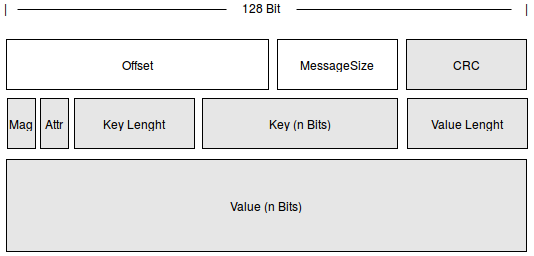
\includegraphics[width=0.7\textwidth]{images/protocol-messageSet.png}
    \caption{Message Set format as common data structure}
    \label{fig:protocol-request-header.png}
\end{figure}

\subsection{Common Request and Response Header}
Each request and response has its same header fields independent for which api they are used. 
The last part of the format (either request or response) is individual to the particular api which is used. 
\begin{figure}[H]
    \centering
    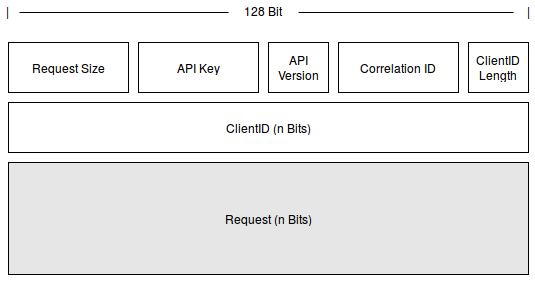
\includegraphics[width=0.7\textwidth]{images/protocol-request-header.png}
    \caption{Common Request Header}
    \label{fig:protocol-request-header.png}
\end{figure}

\begin{figure}[H]
    \centering
    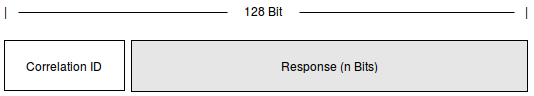
\includegraphics[width=0.7\textwidth]{images/protocol-response-header.png}
    \caption{Common Request Header}
    \label{fig:protocol-response-header.png}
\end{figure}

\subsection{Metadata API}
Describes the currently available brokers, their host and port information, and
gives information about which broker hosts which partitions.

\textbf{Not implemented yet}

\subsection{Produce API}
Send messages to the broker.

\textbf{Not implemented yet}

\subsection{Fetch API}
Fetchs / Consumes messages from the broker.
\subsection{Offset API}
Get information about the available offsets for a given topic partition

\textbf{Not implemented yet}

\subsection{Offset Commit API}
Commit a set of offsets for a consumer group

\textbf{Not implemented yet}

\subsection{Offset Commit API}
Fetch a set of offsets for a consumer group

\textbf{Not implemented yet}

\subsection{Types}

The design of the Apache Kafka protocol allows to make a distinction between three kind of types:
\begin{enumerate}
  \item Related to request
  \item Related to response
  \item Related to data (for either request or response but can also be used for the \fnurl{Apache Kafka Log}{http://kafka.apache.org/documentation.html\#log} component since log files (on-disk) hold the same structure)
\end{enumerate}

As for request and response related types we had to introduce an own naming
convention. As a matter of fact, not every field of some kind of request or
response will be unique. For more than once, there is a field that will
represent a \textit{topicName} for example. Thus, naming the field \textit{
topicName} would have been the obvious solution but since the record syntax in
Haskell won't allow to use the same name for a field twice - even in different
data types - we defined unique prefixes for each request and response as being
listed in the following table:

\begin{table}[h]
\centering
\begin{tabular}{|l|l|l|}
\hline
\textbf{API}            & \textbf{Request (Rq)} & \textbf{Response (Rs)} \\ \hline
Metadata API (Md)       & MetadataRequest       & MetadataResponse       \\ \hline
Produce API (Pr)        & ProduceRequest        & ProduceResponse        \\ \hline
Fetch API (Ft)          & FetchRequest          & FetchResponse          \\ \hline
Offset API (Of)         & OffsetRequest         & OffsetResponse         \\ \hline
Offset Commit API (Ofc) & OffsetCommitRequest   & OffsetCommitResponse   \\ \hline
Offset Fetch API (Oft)  & OffsetFetchRequest    & OffsetFetchResponse    \\ \hline
\end{tabular}
\end{table}

As mentioned before, the representation of the protocol structure is
implemented using the Haskell \fnurl{type
system}{https://wiki.haskell.org/Type}, more concrete using data types created
for our need using the named fields - also known as \fnurl{record
syntax}{http://en.wikibooks.org/wiki/Haskell/More_on_datatypes}.

Given this, a further step of abstraction is introduced by creating types for
the binary representation of a protocol field. The actual type for the data
fields in the protocol have to match an unsigned integer type of its length.
This can easily be done using the
\fnurl{Data.Word}{http://hackage.haskell.org/package/base-4.7.0.2/docs/Data-Word.html}
library. However, while repetitive writing \textit{WordX} (where is stands for
8-, 16-, 32-, or 64 bit) is rather intuitive, creating aliases using the
\textit{type} keyword will result in better readable code, as well as structure
of the implemented protocol.

As a result, a typical data type is described as follows, while details are
hidden for demonstration purposes.:

\begin{lstlisting}
-- more
data Partition =
    ----------------------
    -- ProduceRequest (pr)
    ----------------------
    RqPrPartition
    { rqPrPartitionNumber :: !PartitionNumber
    , rqPrMessageSetSize  :: !MessageSetSize
    , rqPrMessageSet      :: [MessageSet]
    }
    |
    ----------------------
    -- FetchRequest (ft)
    ----------------------
    RqFtPartition
    { rqFtPartitionNumber :: !PartitionNumber
    , rqFtFetchOffset     :: !Offset
    , rqFtMaxBytes        :: !MaxBytes
    }
    |
-- more
\end{lstlisting}

\subsection{Encoding}

\subsection{Decoding}

\section{Network Subsystem}

One of the most fundamental parts of a message broker are sockets. While a
socket is an endpoint of a bidirectional inter-process communication flow, each
connection established to the broker is basically a socket connection. That
being said, it is important to provide a reliable socket server implementation
which will serve correctly under a heavy load. Haskell provides full control
over sockets using the
\fnurl{Network.Socket}{https://hackage.haskell.org/package/network-2.3.0.7/docs/Network-Socket.html}
module which exposes the \fnurl{C socket
API}{http://pubs.opengroup.org/onlinepubs/7908799/xns/syssocket.h.html}.

\subsection{Socket connection establishment}

The following figure (\ref{fig:broker-activity}) shows the abstract view of how
the socket connection between a client and the broker establishes so that a
communication between those two counterparts can proceed.

\begin{figure}[H]
    \centering
    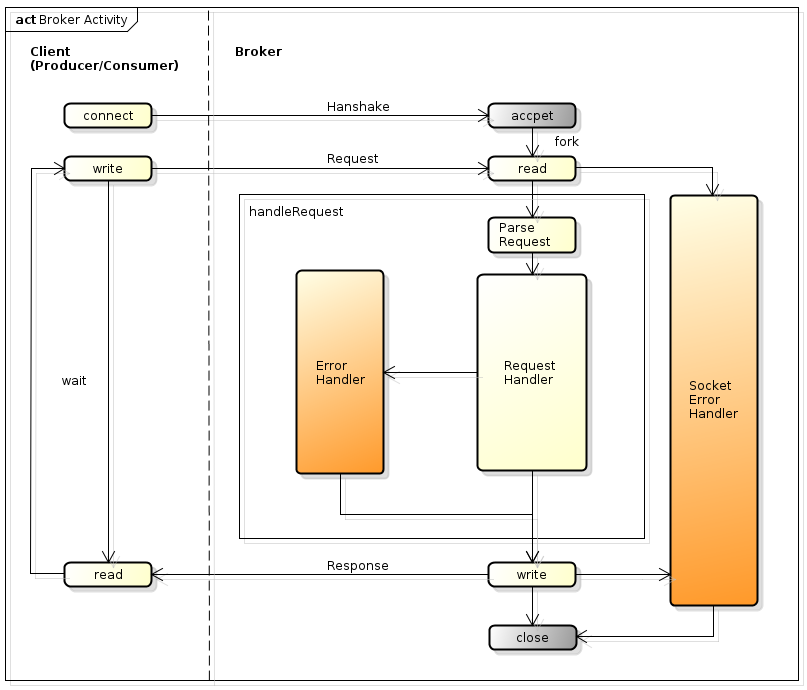
\includegraphics[width=0.7\textwidth]{images/broker-activity.png}
    \caption{Broker request handling concept}
    \label{fig:broker-activity}
\end{figure}

\subsubsection{Create Socket}

First of all, the initialization process of a socket happens on the server by providing the following configuration parameters:
\begin{description}
  \item[Protocol Familiy] \textit{AF\_INET}, for network protocol IPv4
  \item[Socket Type] \textit{Stream}, which provides sequenced, reliable, two-way, connection-based byte streams.
  \item[Protocol Number] \textit{0}, which indicates that the caller does not want to specify the protocol and will leave it up to the service provider.
\end{description}

\subsubsection{Bind Socket}

After the configuration is set, the socket has to be associated with an address
structure which is a constellation of an IP Address and Port. The constructor
\textit{SockAddrInet} of the data type \textit{SockAddr} takes the following
two arguments:

\begin{description}
  \item[Port Number] 4343
  \item[Host Address] iNADDR\_ANY, which binds the socket to all interfaces
\end{description}

TODO: static but could be done with dynamic configuration

\subsubsection{Listen}

While the socket is created and bound to an interface, the socket state can be
entered into listening state. The only configuration parameter which has to be
considered is the maximum number of queued connections they are requesting to
be accepted -- also called backlog. While this parameter is not critical in the
constellation of this broker, we set the queue length to \textbf{50}, which is
also the default value in the Java SocketServer implementation. \textit{Note,
that the focus remains on the amount of data being processed rather than the
number of clients being served.}

\subsection{Receive data}
To receive data from socket buffer we use the function recv from
Network.Socket.ByteString.Lazy library which provides access to the unix socket
interface. Because we work with a binary protocol and need to parse the data
from binary data directly, this module is much more efficient than the string
based network functions. We take the lazy variant of the library because the
input gets directly parsed by our lazy based encoder \todo{ref}.

Because we want to handle each request individually we explicitly read
only the exact amount of bytes which is needed get one particular request from
the socket buffer. To get the size of a whole request we read the first four
bytes which determines the request size according to the protocol and parse it
to an numeral value.

\begin{lstlisting}
import qualified Network.Socket.ByteString.Lazy as S 
import qualified Data.ByteString.Lazy as BL

recvFromSock :: (Socket, SockAddr) -> IO BL.ByteString
recvFromSock (sock, sockaddr) =  do 
    respLen <- S.recv sock (4 :: Int64
    let parsedLen = getLength respLen
    req <- recvExactly sock parsedLength 
    where
        getLength = runGet \$ fromIntegral <\$> getWord32be
\end{lstlisting}

After getting the size of a particular request, this determined amount of bytes
is received from socket. Because of the blocking semantics of unix sockets and
tcp packet fragmentation it is not guaranteed, that the len argument to the recv
system call gets the exactly number of bytes of the whole request. The call may produce
less data than specified. Therefore we implement the following function to get
the data in
chunks until the entire request is read. 

\begin{lstlisting}
recvExactly :: Socket -> Int64 -> IO BL.ByteString 
recvExactly sock size = BL.concat . reverse <\$> loop [] 0 
  where
    loop chunks bytesRead
        | bytesRead >= size = return chunks
        | otherwise = do  
            chunk <- S.recv sock (size - bytesRead)
            if BL.null chunk 
              then return chunks 
              else loop (chunk:chunks) \$! bytesRead + BL.length chunk 
\end{lstlisting}

\subsection{Send data}


\section{API Subsystem (Request Handling)}

\begin{figure}[H]
    \centering
    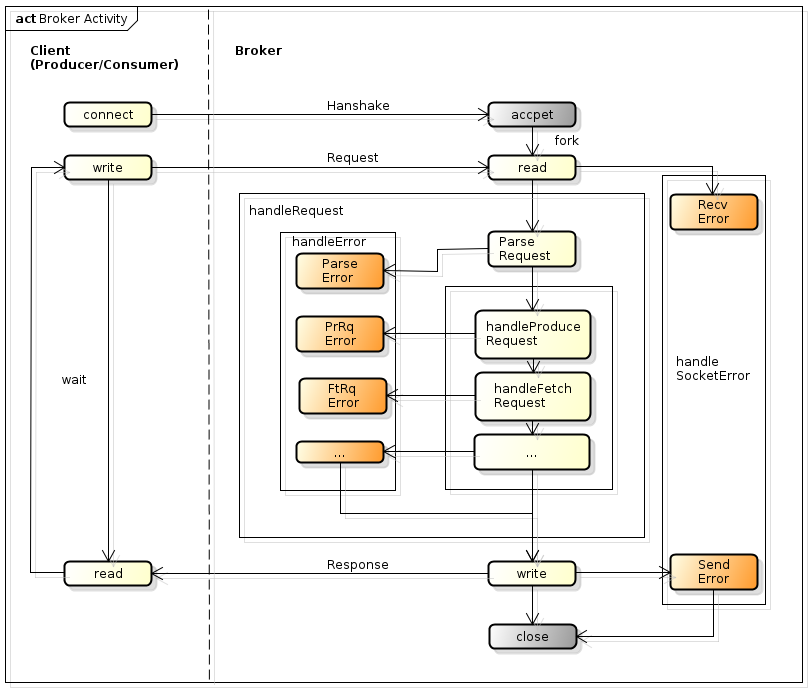
\includegraphics[width=0.7\textwidth]{images/broker-activity-detail.png}
    \caption{Broker request handling concept in detail}
    \label{fig:broker-activity-detail.png}
\end{figure}


\section{Log Subsystem}

\subsection{Indexing}

\subsection{Storage Layout}

- for each topic a folder
- separate folders over partitions (1;2) -> topic\_0; topic\_1
- file name: offset of the first message it contains (next file: S bytes (max log size, given in configuration) from previous file)
- file format: sequence of log entries
- log entry: N (4 byte integer -> message length) followed by message (N message bytes)
- message: unique identifier (64 bit integer offset -> byte position of the start of this message in the stream of all messages ever sent to that topic on that partition)

On-disk format of a message:

offset: 8 bytes
message length : 4 bytes (value: 1+4+n) 
magic value  : 1 byte
crc            : 4 bytes
payload        : n bytes
    ?:              : 1 byte
    ?:              : 4 bytes
    message length  : 4 bytes
    message         : n bytes

\subsection{Types}

\begin{table}[H]
\resizebox{\textwidth}{!}{%
\begin{tabular}{|l|l|l|}
\hline
\textbf{Type synonym} & \textbf{Parameter}           & \textbf{Description}                     \\ \hline
TopicStr              & String                       & Parsed topic name as String              \\ \hline
PartitionNr           & Int                          & Parsed partition number as Int           \\ \hline
FilemessageSet        & {[}MessageSet{]}             &                                          \\ \hline
OffsetIndex           & {[}OffsetPosition{]}         &                                          \\ \hline
LogSegment            & (Log, OffsetIndex)           &                                          \\ \hline
RelativeOffset        & Word32                       & 4 Byte offset relative to the BaseOffset \\ \hline
FileOffset            & Word32                       & 4 Byte physical offset of a Log file     \\ \hline
OffsetPosition        & (RelativeOffset, FileOffset) & Tuple of relative and physical offset    \\ \hline
BaseOffset            & Int                          & 8 Byte offset as Int                     \\ \hline
\end{tabular}
}
\end{table}

\subsection{Write a log}

Writing data, type of MessageSet \todo{ref to type}, to a log is the
fundamental process behind the scenes of handling a ProduceRequest \todo{ref
to request}. But before actually writing data to the file system, several
steps come in between and will contribute significantly to the concept of
Apache Kafka's Log system \todo{ref to kafka log}. This section describes
the implementation details of the mentioned steps in the order of occurrence.

\subsubsection{Base Offset}

The incoming request -- which is at this point already parsed -- contains the
topic as well as the partition number for the given set of messages. Thus, we
can identify the location of the related log file. Given the location only, we yet do
not know which file we actually have to.
The file we want to write to is the one named after the highest offset,
which is why we do not get around reading the content of this directory. While doing so,
string transformations have to be applied to identify the correct offset and thus the
file to write to. Handling the case where no file exists leads
to the creation of a new log with the offset of zero.
\\

Before applying filters and string transformations, the list of files has to be
build. The library
\fnurl{System.Directory}{http://hackage.haskell.org/package/directory-1.2.2.1/docs/System-Directory.html}
provides the function \textit{getDirectoryContents} that takes a file path as a
string and returns a list of all entires in the directory. This operation
performs I/O and thus the return type is an IO monadic value. \textit{As
described on
\fnurl{hackage}{http://hackage.haskell.org/package/directory-1.2.2.1/docs/System-Directory.html\#v:getDirectoryContents},
there are several causes why this operation may fail but at this point, we do
not provide proper error handling.}

Now Haskell can perform it's beauty. To get the list of all offsets within
the directory, the function \textit{offsetFromFileName} extracts the offset
as an \textit{Int} from a \textit{String}. As an example,
\textit{"00000000000000000005.log" :: String } will be transformed to
\textit{0000000000000000005 :: Int}:

\begin{lstlisting}
offsetFromFileName :: [Char] -> Int
offsetFromFileName = read . reverse . snd . splitAt 4 . reverse
\end{lstlisting}

The function \textit{offsetFromFileName} can be mapped over a filtered list of strings, which will
give the list of all offsets within the directory. The filter function
basically omits the files other than the ones ending with \textit{".log"} as well as the root
directories, typically \textit{".", ".."}.


\begin{lstlisting}
getBaseOffsets :: (TopicStr, Int) -> IO [BaseOffset]
getBaseOffsets (t, p) = do
dirs <- getDirectoryContents $ getLogFolder (t, p)
return $ map (offsetFromFileName) (filter (isLogFile) (filterRootDir dirs))
\end{lstlisting}

Finally, the highest offset can be returned. If the list is empty -- and thus no log file 
yet exists within the log folder -- zero will be returned.

\begin{lstlisting}
maxOffset :: [Int] -> Int
maxOffset [] = 0
maxOffset [x] = x
maxOffset xs = maximum xs

getLastBaseOffset :: (TopicStr, Int) -> IO BaseOffset
getLastBaseOffset (t, p) = do
bos <- getBaseOffsets (t, p)
return (maxOffset bos)
\end{lstlisting}

\subsubsection{Offset Position Index}

With the information of the highest offset in the log directory, we do
also now about the currently latest log file.

\subsection{Read from log}

\subsection{Optimization}

Next to optimizations like batching in the network layer \todo{ref to network},
we do also provide some optimizations in terms of I/O. \todo{Kafka: a
Distributed Messaging System for Log Processing}.

\subsubsection{Page Cache:}

First of all, We therefore avoid to explicitly cache messages in memory but
instead rely on the underlying file system cache. This has the benefit of
avoiding double buffering since messages are only cached in the page cache.
Thus, even if the broker process has to be restarted, the cache retains warm.

\todo{more details on modern os and page cache}

\subsubsection{Sequential I/O: }

While producers and consumers lead the broker to access
segments of files, the actual access which taking place is going to be a
sequential access rather than random. This will reduce seeking time to 1 per
partition. In fact, the broker holds a point on a given offset whereas all
messages below the pointer can be considered as already consumed and all
messages with offset greater than the provided one as unconsumed. Now since
messages are ordered this will lead to a sequential I/O with a constant seeking
time (O(1)).


\subsubsection{Internal data transfer:}

As mentioned earlier, HMB omit explicit caching but instead relies on the file system.
Keep this in mind, the actual network access for consumers can be optimized as well.
While a typical approach to sending bytes from a local file to a remote
socket involves the following steps: 
\begin{enumerate}
  \item Read data from storage (disk)
  \item Copy data from the page cache to an application buffer
  \item Copy application buffer to a kernel buffer
  \item Send kernel buffer to the socket
\end{enumerate}

With the help of the sendfile API \todo{ref} it is possible to 
transfer bytes from a file channel to a socket channel, whereas the delivery process will result in the following steps:

\begin{enumerate}
  \item Read data from storage (disk)
  \item Send data from page cache to the socket
\end{enumerate}



\chapter{Evaluation}
\section{Protocol Implementation}
A complete implementation of the Apache Kafka Protocol would
go beyond the scope of this thesis as the focus lies not
only in implementing the protocol but also to provide broker
functionality (see Chapter \ref{chap:broker}). Thus, most important is
the ability to produce and fetch messages. The following list gives 
an overview of what part of the protocol is implemented and what remains open:

\begin{itemize}
    \item Metadata API
    \begin{itemize}
        \tick Topic Metadata Request
        \tick Metadata Response
    \end{itemize}
    \item Produce API
    \begin{itemize}
        \tick Produce Request
        \tick Produce Response
    \end{itemize}
    \item Fetch API
    \begin{itemize}
        \tick Fetch Request
        \tick Fetch Response
    \end{itemize}
    \item Offset API
    \begin{itemize}
        \fail Offset Request
        \fail Offset Response
    \end{itemize}

    \item Offset Commit/Fetch API
    \begin{itemize}
        \fail Consumer Metadata Request
        \fail Consumer Metadata Response
        \fail Offset Commit Request
        \fail Offset Commit Response
        \fail Offset Fetch Request
        \fail Offset Fetch Response
    \end{itemize}
\end{itemize}

The implemented APIs are fully compatible with original Apache Kafka.
Therefore Haskell clients which using the client library of the protocol
implementation (see section \ref{sec:impl-prot-client}), can either communicate
with the HMB or Apache Kafka broker (depending on the set up IP and Port
configuration). 

\newpage
\section{Broker Features}
The scope of this thesis lies on a single broker system with a producer and
consumer API. Therefore it not supports broker replication nor a integration
with Apache Zookeeper like Apache Kafka yet.

\begin{itemize}
    \item Network Layer 
    \begin{itemize}
        \tick Establishing multiple client connections
        \tick Receiving Request over socket
        \tick Sending Responses over socket
    \end{itemize}
    \item API Layer
    \begin{itemize}
        \tick Parsing incoming requests
        \tick Catching and handling errors at runtime 
        \tick Handling Produce requests
        \tick Handling Fetch requests
        \tick Handling Metadata requests
        \fail Handling Offset requests
        \fail Handling Offset Commit/Fetch requests
    \end{itemize}
    \item Producing Messages
    \begin{itemize}
        \tick Publishing messages to specific topic and partition and persist
        them for further consumption
        \tick Support nested sequences of topics, partitions and messages per
        request
        \fail Support configurable Acknowledgements and Timeout
    \end{itemize}
    \item Fetching Messages 
    \begin{itemize}
        \tick Consuming messages of a topic and partition from a specific offset
        on
        \item Support nested sequences of topics and partitions
        \fail Support configurable min and max bytes for fetched data
        \fail Support maximum amount of time to block, waiting if insufficient
        data is available
    \end{itemize}
    \item Accessing Metadata of Topic
    \begin{itemize}
        \tick Requesting metadata for specific topic (or all)
        \tick Responding information about names of available topics
        \tick Responding information about broker instance
        \fail Responding topic or partition specific metadat
        \fail Responding informations about replication 
    \end{itemize}
    \fail Offset Management via Request
    \item Log Persistency
    \begin{itemize}
        \tick Persisting messages in log file
        \tick Guarantee ordering of messages through continuously offsets
        \tick Keep book of a log file with separate index file 
        \fail Log Compaction 
    \end{itemize}
    \item Optimizations 
    \begin{itemize}
        \tick Network throughput 
        \tick Caching
    \end{itemize}
    \fail Message Compression 
    \fail Consumer Groups 
    \fail Broker Recovery
    \fail Broker Replication and Zookeeper Integration
   \end{itemize}

\section{Broker Performance}
-> Test System

Broker Server Setup
\begin{verbatim}
Intel(R) Xeon(R) CPU E3-1245 v3 @ 3.40GHz
One 7200 RPM SATA drive
16GB of RAM
1Gb Ethernet 
\end{verbatim}



-> Durchgeführte Tests 

-> Resultat Network Throuput 

-> Resultat Writing to the log 

-> Vergleich Kafka (ref to Blog) 



\chapter{Conclusion}
\section{Results}
\label{sec:conc-results}
\subsection{Technology Research}
The first result of this thesis is the documentation of the technology research,
which results in gathered knowledge that is further being required for this
thesis.  It gives an insight in messaging fundamentals and  takes a closer look
to Apache Kafka and related topics.

\subsection{Protocol Implementation}

A fundamental result of this thesis is the implementation of the Apache Kafka
protocol in Haskell. The design decision of separating protocol related code
from the broker implementation leads to an isolated product which now can be used
as library for different projects. The code is provided through an \fnurl{open sourced
repository}{https://github.com/hmb-ba/protocol} for further development.

A complete implementation of the Apache Kafka Protocol would go beyond the scope
of this thesis as the focus lies not only in implementing the protocol but also
to provide broker functionality. Thus, most important is the ability to produce
and fetch messages. In order to provide compatibility to Apache Kafka clients
the Metadata API is required too. This is, because it is the first part of the
process of producing or consuming messages whereas it will request information
about the broker and provided topics. The following list gives an overview of
what part of the protocol is implemented and what remains open:

\begin{itemize}
    \item Metadata API
    \begin{itemize}
        \tick Topic Metadata Request
        \tick Metadata Response
    \end{itemize}
    \item Produce API
    \begin{itemize}
        \tick Produce Request
        \tick Produce Response
    \end{itemize}
    \item Fetch API
    \begin{itemize}
        \tick Fetch Request
        \tick Fetch Response
    \end{itemize}
    \item Offset API
    \begin{itemize}
        \fail Offset Request
        \fail Offset Response
    \end{itemize}
    \item Offset Commit/Fetch API
    \begin{itemize}
        \fail Consumer Metadata Request
        \fail Consumer Metadata Response
        \fail Offset Commit Request
        \fail Offset Commit Response
        \fail Offset Fetch Request
        \fail Offset Fetch Response
    \end{itemize}
\end{itemize}

\subsection{Haskell Message Broker}

The main approach of this work is the implementation of a message broker in
Haskell. The resulting application provides a server with basic functionality in
handling requests via network and persisting messages. The broker is fully Kafka
compatible as it is based on the protocol implementation.  In comparison to
original Apache Kafka there are of course a lot of features missing to offer the
same functionality. Furthermore as the scope of this thesis lies on a single
broker system, there is no support for broker replication yet. Nevertheless the
provided Haskell Message broker is a prototype which shows feasibility of
developing a similar system in a fully-fledged functional program language as
Haskell is. The following list gives an overview what features the broker system
already provides and what remains open in the particular area.

Produce API:
\begin{itemize}
        \tick Publishing messages to specific topic and partition
        \tick Publishing to multiple topics and partitions per request
        \tick Support batched messages
        \fail Configurable Acknowledgements and Timeout
\end{itemize}

Fetch API:
\begin{itemize}
        \tick Consuming messages of a specific topic and partition depending on given offset
        \fail Support consuming from multiple topics and partitions per request
        \fail Support configurable min and max bytes for fetched data
        \fail Support consumer groups
        data is available
\end{itemize}

Metadata API:
\begin{itemize}
        \tick Fetching available topic names from broker
        \tick Include broker information
        \fail Include partition status
        \fail Include replication information
\end{itemize}

Persistence (Log):
\begin{itemize}
        \tick Persist messages in topic-partition specific log structure
        \tick Read messages from log, optimized with index file
        \tick Provide LogManager for handling files and directories structure
        \fail Wirte Index to disk and rebuild the memory after the broker is restarted
        \fail Data retention, whereas old data is discarded after fix period of
            time or Kafka's log compaction is applied. 
\end{itemize}

\newpage
\section{Evaluation}

After highlighting the implemented features above, the question about
performance still remains. Is the provided prototype potentially faster than the
original Apache Kafka or has it near the same throughput? Or are we still fare
away from any approximation to the impressive performance of the reference
system? This chapter describes the environment and tools with which the systems
are tested.  It also gives insight in early stress tests which were very useful
in finding network related bugs. Additional benchmarks are defined to
demonstrate the performance of the final version of the Haskell message broker.
For comparison, the original Apache Kafka system is involved to the benchmarks
by running the equivalent tests on same hardware.

\subsection{Test Setup}

The following tests and benchmarks are performed with one the following hardware
setup:

Broker Server:
\begin{verbatim}
Intel(R) Xeon(R) CPU E3-1245 v3 @ 3.40GHz
One 7200 RPM SATA drive
16GB of RAM
1Gb Ethernet 
\end{verbatim}

Client Hardware:
\begin{verbatim}
Intel(R) Core(TM) i7-2720QM CPU @ 2.20GHz
One SSD SATA drive
16GB of RAM 
1Gb Ethernet
\end{verbatim}

\subsection{HMB Performance Producer}
\label{conc-eval-hmbperformanceprod}

The HMB performance producer is a simple console application used for stress
tests to the broker system. It can be used to generate messages of a given size
and batch them into a single request. It then repeatedly calls the client
library function sendRequest to pack, encode and send the request. The following
code shows the simplified main function:

\begin{lstlisting}
import qualified System.Entropy as E

main = do 
    -- Socket setup 
    -- ....

    -- Get numberOfBytes and batchSize as variable input 
    -- ....

    randBytes <- E.getEntropy numberOfBytes 
    let batch = [randBytes | x <- [1..batchSize]]

    replicateM_ 1000000 (sendRequest sock req) 
    putStrLn "done produce"
    return ()

\end{lstlisting}

\subsection{Kafka Performance Producer}
\label{conc-eval-kafkaperformanceprod}

The \fnurl{Kafka Performance Producer}
{https://github.com/apache/kafka/blob/trunk/clients/src/main/java/org/apache/kafka/clients/tools/ProducerPerformance.java}
is a official product of Apache Kafka to systematically test their broker
system. It is a wrapper around the original Kafka producer client for producing
as much messages as possible. It provides many \fnurl{configuration options}
{http://kafka.apache.org/documentation.html\#newproducerconfigs} for specific
benchmarks. Because the Haskell message broker offers Kafka compatibility, this
performance producer can also be used as an alternative to the HMB performance
producer to test.

The following listing shows the setup for the benchmarks of this thesis, values
in in brackets [ ] are placeholders for the relevant parameters for the
benchmarks.

\begin{verbatim}
Start Zookeeper
>bin/zookeeper-server-start.sh config/zookeeper.properties

Start Kafka Node 
> bin/kafka-server-start.sh config/server.properties

Create Test Topic [TopicName] on broker server with [IP], 
one partition, no replication: 
>bin/kafka-topics.sh --zookeeper [IP]:2181 
    --create --topic [TopicName] --partitions 1 --replication-factor 1

Start single threaded producing benchmark: 
> bin/kafka-run-class.sh org.apache.kafka.clients.tools.ProducerPerformance 
    [TopiName] [NumberOfMessages] [MessageSize] -1 acks=1 
    bootstrap.servers=[IP]:[Port] buffer.memory=67108864 batch.size=[BatchSize]
\end{verbatim}


%\subsection{Test tools}
%\subsubsection{Wireshark}
%Wireshark is used to track tcp streams of ongoing network communication. For the
%To test network throughput and analyze transmitted tcp packaged the tool
%Wireshark is used. 

%\begin{figure}[H]
%    \centering
%    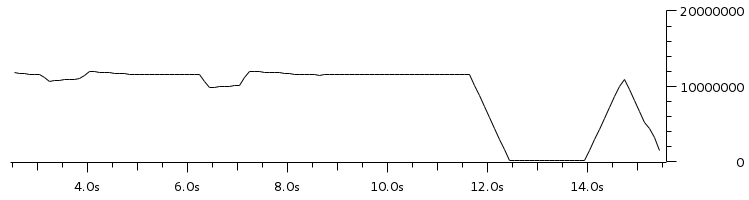
\includegraphics[width=0.85\textwidth]{images/benchmark/bench-1000-1-eth.png}
%    \caption{Example getting tcp throughput graph for specific benchmark test}
%\end{figure}

%\subsubsection{Iptraf-ng}

\newpage
\subsection{Early stress tests}

An early version of the broker provided a console client which produced messages
per console input. This setup demonstrated that encoding/decoding of a request
worked. Also the different broker layers have done their job well.  Later in the
construction phase of the broker, tests which repeatedly send a large amount of
requests in short period of time where introduced. This kind of stress test is
very useful to test network related bugs and performance lacks. The following
table lists some of the major issues, that were exposed: 

\begin{table}[H]
\begin{tabular}{|p{4cm}|p{5cm}|p{6cm}|}
\hline
{\bf Exposed Issue}                                                                                  & {\bf Cause}                                                                                                                                                                                                                 & {\bf Solution}                                                                                                                                                                                                                                                                                    \\ \hline
Dramatically slowdown after short period of time                                                       & TCP Zero Window - Socket receive buffer of broker full                                                                                                                                                                      & Broker application was to slow in receiving, parsing and handling incoming requests. Threading concept need to be optimized (see \ref{sec:impl-broker-threading}). The process of parsing an incoming request need to be swap out to another thread, so that the network receive thread can reduce socket buffer fast enough. \\ \hline
Parsing from socket error "not enough bytes"  when testing over network
interface instead of loopback. & The \lstinline{len} argument to the
\lstinline{recv} system call is merely the upper bound on the received length
(e.g. the size of the target buffer); the call may produce less data than asked
for & Introduced function which checks if really the exact amount of bytes is
read. If not, the \lstinline{recv} call is repeated until all requested bytes are present (see details in \ref{sec:impl-broker-socket-receive}).                                                                                                                                              \\ \hline
Throughput drop when producing larger request with nested list
& Issue in encoding a request, called \lstinline{runPut} on each sub element and
appended to a whole.
& No appending of parsed sub elements. Restructure encode module by running
\lstinline{runPut} at latest point in time. This resulted in factor 2 of performance in building requests (see \ref{sec:impl-prot-encoding}).                                                                                                                                      \\ \hline
Very slow performance in persisting messages to the log (file system).                                 & No state and batching at broker side. Each incoming message ended in multiple file accesses which slowed down the whole process.                                                                                                                                & Messages need to be sum up to larger chunks of bytes. After defined period of time or amount of bytes, multiple messages need to be flushed to disk at once (see details of different approaches in \ref{sec:impl-broker-log}).                                                                                                                                      \\ \hline
\end{tabular}
\end{table}
\captionof{table}{Uncovered issues in early stress tests}


\subsection{Profiling}
When dealing with thousands of request per seconds, function with high complexity
can cause terribly bottlenecks. A method to analyze Haskell code for
potentially slow functions is time and allocation profiling provided by GHC.

TODO
-- Setup?
-- Results 

\subsection{Producer Benchmark "Effect of Message Batch size"}
\label{sec:conc-benchmark-1}

The goal of this benchmark is to analyze the network throughput between producer
client and broker system.  The focus lies on the effect of changing the batch
size at producer client to the resulting transmission of bytes per second. The
batch size determines the amount of bytes for which messages will be packed
together and sent to broker as single request for efficiency.  Increasing the
batch size requires more memory. The size of a single message is fixed to 100
bytes, because it is the more interesting case for a messaging system
(generally). It is easy to get good throughput in MB/sec if the messages are
large, but much harder to get good throughput when the messages are small, as
the overhead of processing each message dominates.

Calculation batch size in bytes:
\begin{verbatim}
    Messages Batched * (Message Size + Message Overhead) + Request Overhead 
\end{verbatim}

\subsubsection{Conditions}
\begin{table}[H]
\begin{tabular}{|l| p{12cm}|} \hline
{\bf Message Size}   & 100 Bytes \\ \hline
{\bf Batch Size [B]} & 195 | 1000 | 8192 | 16384 (Kafka default) | 56769 \\ \hline
{\bf Tested Clients} &
    \begin{itemize}
        \item Kafka PerformanceProducer 2.10-0.8.2.0, single threaded
        \item HMB Producer, single threaded
    \end{itemize}\\ \hline
{\bf Tested Brokers} &
    \begin{itemize}
        \item Kafka Broker 2.10-0.8.2.0, no replication, one partition
        \item HMB Broker, no replication, one partition
    \end{itemize}\\ \hline
{\bf Measurement} & Resulting TCP throughput over a period of 10 seconds, analyzed with
    Wireshark. \\ \hline
{\bf Scenarios} & Producing as much messages as possible from client (left) to broker (right).
    The size of messages batched together varies in defined steps.
    \begin{enumerate}
        \item Kafka Performance Producer $\rightarrow$ Kafka Broker
        \item Kafka Performance Producer $\rightarrow$ HMB Broker
        \item HMB Producer $\rightarrow$ Kafka Broker
        \item HMB Producer $\rightarrow$ HMB Broker
    \end{enumerate} \\ \hline
\end{tabular}
\end{table}
\captionof{table}{Benchmark conditions "Effect of Producer Batch size"}
\newpage
\subsubsection{Results}
The results fora each specific scenarios are given below. The graph shows the
TCP throughput in bytes in period of ten to twenty seconds.

Scenario 1, Kafka $\rightarrow$ Kafka:

\begin{table}[H]
\centering
\begin{tabular}{|l|l|l|} \hline
195 (1 Msg) & 1387 ($\sim$10 Msgs)& 8192 ($\sim$65 Msgs)\\ \hline
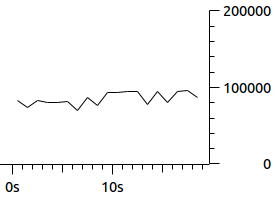
\includegraphics[width=0.25\textwidth]{images/benchmark-1/benchmark-1-s1-bs195.png}
&
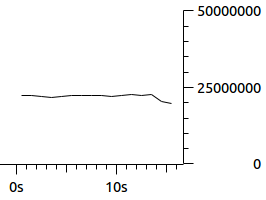
\includegraphics[width=0.25\textwidth]{images/benchmark-1/benchmark-1-s1-bs1387.png}
&
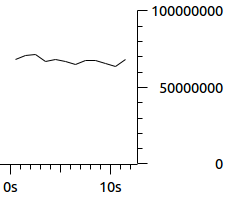
\includegraphics[width=0.2\textwidth]{images/benchmark-1/benchmark-1-s1-bs8192.png} \\ \hline
\end{tabular}
\end{table}

\begin{table}[H]
\centering
\begin{tabular}{|l|l|} \hline
16384 ($\sim$130 Msgs)& 56769 ($\sim$450 Msgs)\\ \hline
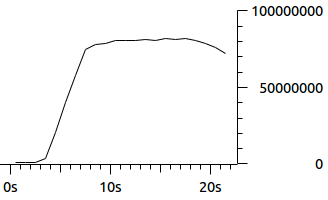
\includegraphics[width=0.25\textwidth]{images/benchmark-1/benchmark-1-s1-bs16384.png}
&
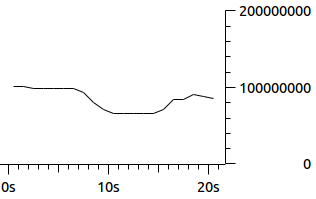
\includegraphics[width=0.25\textwidth]{images/benchmark-1/benchmark-1-s1-bs56769.png} \\ \hline
\end{tabular}
\end{table}

Scenario 2, Kafka $\rightarrow$ HMB:

\begin{table}[H]
\centering
\begin{tabular}{|l|l|l|} \hline
195 (1 Msg) & 1387 ($\sim$10 Msgs)& 8192 ($\sim$65 Msgs)\\ \hline
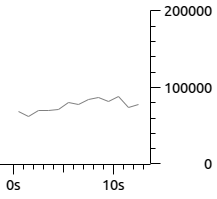
\includegraphics[width=0.2\textwidth]{images/benchmark-1/benchmark-1-s2-bs195.png}
&
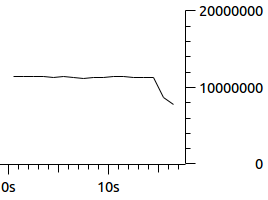
\includegraphics[width=0.25\textwidth]{images/benchmark-1/benchmark-1-s2-bs1387.png}
&
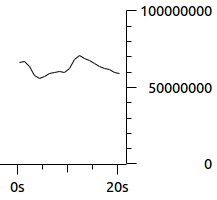
\includegraphics[width=0.2\textwidth]{images/benchmark-1/benchmark-1-s2-bs8192.png} \\ \hline
\end{tabular}
\end{table}

\begin{table}[H]
\centering
\begin{tabular}{|l|l|} \hline
16384 ($\sim$130 Msgs)& 56769 ($\sim$450 Msgs)\\ \hline
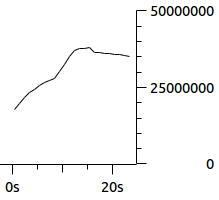
\includegraphics[width=0.2\textwidth]{images/benchmark-1/benchmark-1-s2-bs16384.png}
&
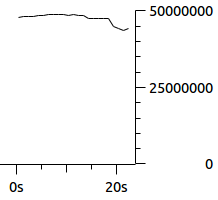
\includegraphics[width=0.2\textwidth]{images/benchmark-1/benchmark-1-s2-bs56769.png} \\ \hline
\end{tabular}
\end{table}

\newpage
Scenario 3, HMB $\rightarrow$ Kafka:

\begin{table}[H]
\centering
\begin{tabular}{|l|l|l|} \hline
195 (1 Msg) & 1387 ($\sim$10 Msgs)& 8192 ($\sim$65 Msgs)\\ \hline
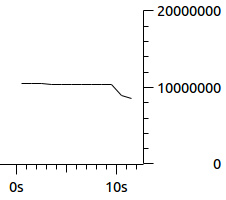
\includegraphics[width=0.2\textwidth]{images/benchmark-1/benchmark-1-s3-bs200.png}
&
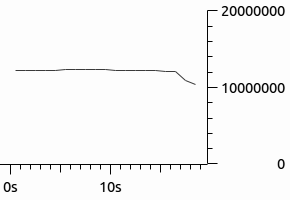
\includegraphics[width=0.25\textwidth]{images/benchmark-1/benchmark-1-s3-bs1400.png}
&
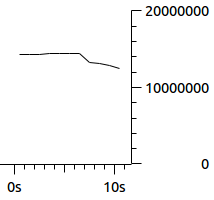
\includegraphics[width=0.2\textwidth]{images/benchmark-1/benchmark-1-s3-bs8192.png} \\ \hline
\end{tabular}
\end{table}

\begin{table}[H]
\centering
\begin{tabular}{|l|l|} \hline
16384 ($\sim$130 Msgs)& 56769 ($\sim$450 Msgs)\\ \hline
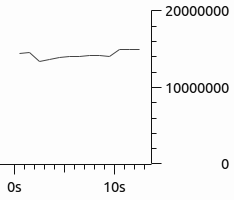
\includegraphics[width=0.2\textwidth]{images/benchmark-1/benchmark-1-s3-bs16384.png}
&
\includegraphics[width=0.2\textwidth]{images/benchmark-1/benchmark-1-s3-bs56769.png} \\ \hline
\end{tabular}
\end{table}

Scenario 4, HMB $\rightarrow$ HMB:

\begin{table}[H]
\centering
\begin{tabular}{|l|l|l|} \hline
195 (1 Msg) & 1387 ($\sim$10 Msgs)& 8192 ($\sim$65 Msgs)\\ \hline
\includegraphics[width=0.2\textwidth]{images/benchmark-1/benchmark-1-s4-bs195.png}
&
\includegraphics[width=0.25\textwidth]{images/benchmark-1/benchmark-1-s4-bs1387.png}
&
\includegraphics[width=0.2\textwidth]{images/benchmark-1/benchmark-1-s4-bs8192.png} \\ \hline
\end{tabular}
\end{table}

\begin{table}[H]
\centering
\begin{tabular}{|l|l|} \hline
16384 ($\sim$130 Msgs)& 56769 ($\sim$450 Msgs)\\ \hline
\includegraphics[width=0.2\textwidth]{images/benchmark-1/benchmark-1-s4-bs16384.png}
&
\includegraphics[width=0.2\textwidth]{images/benchmark-1/benchmark-1-s4-bs56769.png} \\ \hline
\end{tabular}
\end{table}

\newpage
\subsubsection{Conclusion}
\begin{table}[H]
\centering
\begin{tabular}{|l|l|l|l|l|}
\hline
{\bf Benchmark Variable} & \multicolumn{4}{c|}{{\bf Avg. Throughput {[}MB/s{]}}} \\ \hline \hline
Batch Size [Byte]        & Scenario 1       & Scenario 2       & Scenario 3   & Scenario 4   \\ \hline
195  (1 Msg)             & 9                & 8                & 10           & 9            \\ \hline
1387 ($\sim$10 Msgs)     & 24               & 12               & 11           & 16           \\ \hline
8192 ($\sim$65 Msgs)     & 68               & 54               & 13           & 15           \\ \hline
16384 ($\sim$130 Msgs)   & 80               & 32               & 14           & 16           \\ \hline
56769 ($\sim$450 Msgs)   & 98               & 48               & 16           & 17           \\ \hline
\end{tabular}
\end{table}
\captionof{table}{Results of benchmark "Effect of Producer Batch size"}

The result of this benchmark demonstrates the positive effect to the throughput
by increasing the producing batch size. The original Kafka setup (scenario 1),
shows a significant rise by increasing the batch size. However the
HMB setup (scenario 4) cannot use batching to full capacity. Obviously this
benchmark exposes the HMB producer as major bottleneck. Using the Kafka
producer to the HMB broker (scenario 2) gives lot better results instead of
using the HMB producer. Scenario 3 approves this suspicion. The handling
of requests on the HMB broker is quite efficient but there is still a demand
for further optimizations to get same performance than Kafka.

\subsubsection{Consequences}
During the benchmark it was conspicuous that the HMB broker is
not using full capacity of CPU. While Kafka is obviously getting use of
multi-threading, at HMB the most load weigh on a single thread. This is why
there is only one API handler thread running at the time, which is definitely
a point to optimize in future.

TODO: Figure of CPU workload

Another point with demand to optimization is the producer which manifests a
bottleneck with messages of 100 bytes (when the message size gets bigger, the
result is much better! ref). Because the provided HMB producer is quite simple
(actually just built to test), another task for the futur is to work off details for
optimized producer client which would definitely lead to better results. 

\newpage
\subsection{Producer Benchmark "Effect of Message size"}
\label{sec:conc-benchmark-2}
The goal of this benchmark is to analyze the network throughput between
producer client and broker system. The focus lies on the effect of changing the
size of a single message to the resulting transmission of bytes per
second. Persisting performance on the broker is not considered in
this benchmark.

\subsubsection{Conditions}
\begin{table}[H]
\begin{tabular}{|l| p{12cm}|} \hline
{\bf Message Size}   & 10 | 100 | 1000 | 10000 | 100000 | Bytes \\ \hline
{\bf Batch Size}     & 12800 \\ \hline
{\bf Tested Clients} &
    \begin{itemize}
        \item Kafka PerformanceProducer 2.10-0.8.2.0, single threaded
        \item HMB Producer, single threaded
    \end{itemize}\\ \hline
{\bf Tested Brokers} &
    \begin{itemize}
        \item Kafka Broker 2.10-0.8.2.0, no replication, one partition
        \item HMB Broker, no replication, one partition
    \end{itemize}\\ \hline
{\bf Measurement} & Resulting TCP throughput over a period of 10 seconds, analyzed with
    Wireshark. \\ \hline
{\bf Scenarios} & Producing as much messages as possible from client (left) to broker (right).
    The size of a messages varies in defined steps. The batch size thereby is a fixed value. 
  \begin{enumerate}
        \item Kafka Performance Producer $\rightarrow$ Kafka Broker
        \item Kafka Performance Producer $\rightarrow$ HMB Broker
        \item HMB Produer $\rightarrow$ Kafka Broker
        \item HMB Produder $\rightarrow$ HMB Broker
    \end{enumerate} \\ \hline
\end{tabular}
\end{table}
\captionof{table}{Benchmark conditions "Effect of Message size"}

\subsubsection{Results}
\begin{table}[H]
\centering
\begin{tabular}{|l|l|l|l|l|}
\hline
{\bf Benchmark Variable} & \multicolumn{4}{c|}{{\bf Avg. Throughput {[}MB/s{]}}} \\ \hline
Message Size             & Scenario 1       & Scenario 2       & Scenario 3     & Scenario 4 \\ \hline
10 B                     &                  &                  & 0              &           \\ \hline
100 B                    & 0                & 0                & 0              &            \\ \hline
1000 B (1 KB)            & 0                & 0                & 0              &            \\ \hline
10000 B (10 KB)          & 0                & 0                & 0              &            \\ \hline
100000 B (100 KB)        & 0                & 0                & 0              &             \\ \hline
1000000 (1 MB)           & 0                & 0                & 0              &             \\ \hline
\end{tabular}
\end{table}
\captionof{table}{Results of benchmark "Effect of Message size"}

%\subsection{Benchmark "Encode/Decode"}

%\subsection{Network Throughput}
%The socket based communication must not be a bottleneck in a high performance
%broker. A producer should be able to send with near the maximal throughput of
%its local network card, whereas the broker needs to handle the incoming data
%streams as fast as possible. If the limits of a single network connection is
%reached, the next step to improve performance is to balance the data
%stream on multiple replicated brokers.

%To test the network throughput for this thesis, a benchmark producer
%which identify the limits is provided.



%The variance seems to be due to Linux's I/O management facilities that batch
%data and then flush it periodically.
%-> Durchgeführte Tests 

%-> Resultat Network Throuput 

%-> Resultat Writing to the log 
%-> Vergleich Kafka (ref to Blog) 

%\begin{table}[h]
%\begin{tabular}{|c|c|c|c|}
%\hline
%{\bf Request Size (with ReqHeader)} & {\bf Message Size {[}Byte{]}} & {\bf Batch Size} & {\bf \begin{tabular}[c]{@{}c@{}}Avg. Throughput\\ {[}MB/s{]}\end{tabular}} \\ \hline
%150 B                               & 100                           & 1                & 27                                                                         \\ \hline
%1050 B                              & 100                           & 10               & 22                                                                         \\ \hline
%10.050 KB                           & 100                           & 100              & 30                                                                         \\ \hline
%100.050 KB                          & 100                           & 1000             & 32                                                                         \\ \hline
%1 MB                                & 100                           & 10000            & 40                                                                         \\ \hline
%550 B                               & 500                           & 1                & 66                                                                         \\ \hline
%1050 B                              & 500                           & 2                & 81                                                                         \\ \hline
%10.050 B                            & 500                           & 20               & 80                                                                         \\ \hline
%100.050 KB                          & 500                           & 200              & 96                                                                         \\ \hline
%1 MB                                & 500                           & 2000             & 68                                                                         \\ \hline
%1050 B                              & 1000                          & 1                & 104                                                                        \\ \hline
%10.050 B                            & 1000                          & 10               & 110                                                                        \\ \hline
%100.050 KB                          & 1000                          & 100              & 112                                                                        \\ \hline
%1 MB                                & 1000                          & 1000             & 87                                                                         \\ \hline
%10.050 B                            & 10000                         & 1                & 117                                                                        \\ \hline
%100.050 KB                          & 10000                         & 10               & *                                                                          \\ \hline
%1 MB                                & 10000                         & 100              & *                                                                          \\ \hline
%\end{tabular}
%\end{table}


\section{Outlook}

What are the next steps? As described in section \ref{sec:conc-results}, the
resulting broker implementation is not a finalized product -- it is a prototype.
It shows that it is feasible to develop an Apache Kafka like broker system
written in Haskell. An extendable and scalable implementation base and
architecture is provided. The provided benchmarks (\ref{sec:conc-benchmark-1}
and \ref{sec:conc-benchmark-2}) demonstrate good performance put also uncover
some major bottlenecks. We are certain that with further work one could build
the current version to an extraordinary broker system.

Summarized, the next tasks to do at the prototype would involve:
\begin{enumerate}
    \item Facing uncovered bottlenecks (see benchmarks)
    \item Implementation and handling of remaining API's
    \item Extending the log subsystem
    \item Work off more details for Client API
    \item Further optimizations
\end{enumerate}

After bringing the broker server to a stable and nearly feature complete
application, the next step would be to introduce broker replication. This task
probably is predestined for a further thesis whereas the goal is to analyze
distributed replication in detail and work out ZooKeeper
integration.

The Haskell community is very vital and active. We experienced that at the
\fnurl{ZuriHac 2015}{https://wiki.haskell.org/ZuriHac2015} (Google Zurich,
29.05.15) or \fnurl{HaskellerZ Meetup}{http://www.meetup.com/de/HaskellerZ/}
(ETH Zurich, 30.04.2015) we have participated during this thesis. The results
of this work will still be published open source through the \fnurl{GitHub
repositories}{https://github.com/hmb-ba}. The goal is to find contributors for
further development. For this reason we will also present this work in a
separate Meetup later in summer 2015. As for now, the highlight remains the
protocol implementation which has already been praised by the Haskell community
and found its contributors they helped uncovering minor issues.



\cleardoublepage


\begin{appendices}
% Für eprints auskommentieren <<<
% \chapter{Erklärung zur Urheberschaft}

Die vorliegende Arbeit basiert auf Ideen, Arbeitsleistungen, Hilfestellungen
und Beiträgen gemäss folgender Aufstellung:

\begin{tabular}[l]{| p{8cm} | l | l |}
\hline
\textbf{Gegenstand, Leistung} & \textbf{Person} & \textbf{Funktion} \\ \hline \hline
\begin{itemize}
  \item \ldots
\end{itemize}
  & Emanuel Duss
  & Autor der Arbeit \\ \hline
\begin{itemize}
  \item \ldots
\end{itemize}
  & Roland Bischofberger
  & Autor der Arbeit \\ \hline
\begin{itemize}
  \item \ldots
\end{itemize}
  & Cyrill Brunschwiler
  & Betreuer, Industriepartner \\ \hline
\end{tabular}

Die hier nicht explizit erwähnten Teile wurden zusammen erarbeitet.

Ich erkläre hiermit,

\begin{itemize}
  \item dass ich die vorliegende Arbeit gemäss obiger Zusammenstellung selber
    und ohne weitere fremde Hilfe durchgeführt habe,
  \item dass ich sämtliche verwendeten Quellen erwähnt und gemäss gängigen
    wissenschaftlichen Zitierregeln korrekt angegeben habe,
  \item dass in der Arbeit verwendete urheberrechtlich geschützte (Copyright)
    Inhalte (insbesondere Fotografien und Grafiken) klar gekennzeichnet und mit
    Quellenhinweis versehen sind,
  \item dass Inhalte die unter Creative-Commons-Lizenz veröffentlicht wurden,
    klar gekennzeichnet sind.
\end{itemize} 

% \begin{figure}[H]
%   \centering
%   \includegraphics[width=15cm]{images/urheberschaft_unterschrift.png}
% \end{figure}

% \include{vereinbarung_weiterentwicklung}
% \chapter{Persönliche Berichte}

\section{Bericht: Marc Juchli}

\subsection{Aufgabenstellung}
\subsection{Teamarbeit}
\subsection{Negative Erfahrungen}
\subsection{Positive Erfahrungen}


\section{Bericht: Lorenz Wolf}

\subsection{Aufgabenstellung}
\subsection{Teamarbeit}
\subsection{Negative Erfahrungen}
\subsection{Positive Erfahrungen}

% <<<
\chapter{Projectmanagement}

\section{Introduction}

\subsubsection*{Purpose of this document}
This chapter shows the project plan for the bachelor thesis "Functional Kafka".
It is used as basis for the planning during the work. 

\subsubsection*{Goal of the project}
Analyzing Apache Kafka, a state of the art message broker system created at
LinkedIn and adapt basic features to build an alternative broker system in
Haskell. 

\section{Organization}

\subsubsection*{Structure}

\begin{tabular}[t]{|l|l|l|} \hline
\textbf{Name} & \textbf{E-mail} & \textbf{Responsibility} \\ \hline
Marc Juchli & mjuchli@hsr.ch & Research, Development, Documentation \\ \hline
Lorenz Wolf & l1wolf@hsr.ch & Research, Development, Documentation \\ \hline 
\end{tabular}

\subsubsection*{Externe Schnittstellen}

\begin{tabular}[t]{|l|l|l|} \hline
\textbf{Name} & \textbf{E-Mail} & \textbf{Responsibility}  \\ \hline
Prof Dr. Josef Joller & jjoller@hsr.ch & Supervisor \\ \hline 
Dr. Simon Meier & simon.y.meier@gmail.com & Expert  \\ \hline\end{tabular}

%\subsubsection*{Sitzungen}

%\begin{itemize}
%\item 
%\end{itemize}
\newpage
\section{Planning}
We separated the work in three phases inception, elaboration and construction
(adapted from Rational Unified Process, RUP). For planning the time schedule we
first defined tasks very rough granular. For each of those we then planed
subtasks which can be seen as single issues (see \ref{subsec:tasks}).
Furthermore three milestones were set to define particular objectives we want to
achieve at a specific time (see table \ref{tab:MeilensteineZiele}).  After reaching the
planed end of a milestone, a set-actual comparison is made (see
\ref{sec:status-tracking}). Performed work is
tracked via an Atlassian JIRA platform where we manage tasks for the project. 


\subsection{Time schedule}
\begin{figure}[H]
    \centering
    \includegraphics[width=1\textwidth]{images/workschedule.png}
    \caption{Time schedule, GANTT style}
    \label{fig:workschedule}
\end{figure}

\subsection{Milestones}
\begin{tabular}[H]{|p{4cm}|l|p{4.5cm}|p{4.5cm}|}\hline
    \textbf{Milestone} & \textbf{Deadline} & \textbf{Objectives} & \textbf{Deliverables} \\ \hline
    M0 Start of work & 16.02.2015 & - & -\\ \hline
    M1 Completion of research  & 22.03.2015 & 
        Necessary background knowledge about Kafka related topics as well as
        Haskell skills are ready for implementation part. 
        &
        Documentation technology research \\ \hline
    M2 End of elaboration & 19.04.2015 & 
        After a period of three weeks we want to have a concept and first running
        code to show some basic functionality and feasibility. 
        &
        Architecture prototype \\ \hline
    M3 End of construction & 07.06.2015 & 
        Code freeze, all planned features are implemented. Broker runs stable and
        benchmark results exist. 
        &
        Stable broker and protocol implementation. Benchmarks results. \\ \hline
  %\begin{itemize}
  %  \item \ldot
  %\end{itemize} \\ \hline
\end{tabular}
\captionof{table}{Milestones and their objectives}
\label{tab:MeilensteineZiele}

\newpage
\subsection{Tasks}
\label{subsec:tasks}
\subsubsection{Inception}


\begin{tabular}[H]{|p{6cm}|p{10cm}|}\hline
    \textbf{Task} & \textbf{Subtasks} \\ \hline
    Technology Research Kafka & 
        \begin{itemize}
            \item Learn Messaging and Event Streaming fundamentals.
            \item Analyse Apache Kafka and related topics. 
            \item Write research documentation.
        \end{itemize} \\ \hline
    Practice programming Haskell & 
        \begin{itemize}
            \item Familiarize with the functional paradigm.
            \item Setup developer environment and repositories. 
            \item Learn Haskell as functional programming language.
            \item Become acquainted to libraries regarding networking,
              building server application, and serialization.
        \end{itemize} \\ \hline
\end{tabular}
\captionof{table}{Tasks of inception phase}

\subsubsection{Elaboration}
\begin{tabular}[H]{|p{6cm}|p{10cm}|}\hline
   \textbf{Task} & \textbf{Subtasks} \\ \hline
    Architecture Prototype &
        \begin{itemize}
            \item Set up basic server architecture.
            \item Set up concept for implementing the wire protocol.
            \item Implement basic message workflow from producing messages and
            persisting at broker to consuming the data from another clients.
            \item Implement simplified clients to demonstrate architecture
                prototype prototype.
        \end{itemize} \\ \hline
   \end{tabular}
\captionof{table}{Tasks of elaboration phase}

\subsubsection{Construction}
\begin{tabular}[H]{|p{6cm}|p{10cm}|}\hline
   \textbf{Task} & \textbf{Subtasks} \\ \hline
    Protocol Implementation &
        \begin{itemize}
            \item Build standalone package providing an independent Kafka
                protocol library.
            \item Work out details of protocol implementation. Finish
                implementation of relevant parts for producing and consuming
                messages. 
            \item Implement client API for exposing simplified access to protocol
                implementation.
            \item Test Kafka compatibility.
        \end{itemize} \\ \hline
    Broker Implementation &
        \begin{itemize}
            \item Work out server application handling multiple connections
            sending produce or consume requests.
            \item Develop message log persistency adapt from Apache Kafka. 
            \item Optimize performance to approximate performance approach of
            Apache Kafka. 
        \end{itemize} \\ \hline
    Benchmarking &
        \begin{itemize}
            \item Test resulting broker implementation for performance.
            \item Comparing performance with Apache Kafka.
        \end{itemize} \\ \hline
\end{tabular}
\captionof{table}{Tasks of construction phase}

Last week of the schedule is reserved for completion work and documentation. 


\newpage
\section{Risk management}

In the table \ref{tab:Risiken} are the risk which could influence our thesis: 

\begin{tabular}[t]{|p{3cm}|p{3cm}|r|r|r|p{3cm}|p{3cm}|}\hline
\textbf{Risk} &
    \textbf{Impact} &
  \begin{sideways} \textbf{Probability } \end{sideways} &
  \begin{sideways}\textbf{Loss} \end{sideways} &
  \begin{sideways}\textbf{Risk} \end{sideways} &
  \textbf{Prevention} & \textbf{Consequences} \\ \hline
    Missing know-how in new technology & 
    Slow progress, inefficiency & 
    0.9 & 
    0.1 & 
    0.3 & 
    Ask experts before spending to much time & 
    It is part of this thesis to learn new technologies, we expect decelerated
    progress from time to time but we can deal with it. \\ \hline
  Technical impossibility & 
    No resulting product, change to other technology, loss in time. & 
    0.1 & 
    0.9 & 
    0.1 & 
    Analyse possibilities before spending to much time . &
    Inform supervisor or expert.
    \\ \hline
\end{tabular}
\captionof{table}{Risks}
\label{tab:Risiken}

%Sollte trotz den vorbeugenden Massnahmen ein zeitlicher Schaden
%entstehen, muss die Projektplanung unter Umständen angepasst werden.
%Die Zeiterfassung wird von den Projektmitarbeitern in Redmine erfasst.
%Redmine ist über folgenden Link erreichbar:
%\url{http://152.96.56.42/redmine/}. Die Projektmitarbeiter haben einen
%persönlichen Zugang  um die Daten zu erfassen. Der Betreuer hat
%ebenfalls ein Zugang, mit welchem er die Fortschritte mitverfolgen kann.
%Auf Redmine ist der aktuelle Stand des Projekts zu sehen.


%\section{Qualitätsmanagement}

%Um die Arbeitsergebnisse qualitativ auf einem hohen Niveau zu halten,
%arbeiten die Projektmitglieder nach dem Vier-Augen-Prinzip. Ein Dokument
%wird immer von beiden durchgelesen. Allfällige Änderungen werden gleich
%bilateral diskutiert und allenfalls angebracht. Somit soll erreicht
%werden, dass beide Projektmitglieder mit den Ergebnissen einverstanden
%und zufrieden sind.  Um Programmieraufgaben durchzuführen, kann
%teilweise der Ansatz von Pairprogramming eingesetzt werden. Dies führt
%dazu, dass sich beide mit dem Code auskennen.

\section{Status Tracking}
\label{sec:status-tracking}

\subsection{Milestone 1}
Milestone one was reached at 22.03.2015 by finishing the technology research
phase of our thesis. We delivered the resulting documentation, where we discuss
Messaging, Event Streaming and Apache Kafka as reference system. Originally we
had the idea to make a detailed survey about alternatives to Apache Kafka by
trying to compare them. After intensively analyzing different systems we
realized that it need much more time to give well-founded statements. Because we
wanted to comply the project plan an we had not much time anymore, we decided to
cut this part of the research documentation. This past six weeks were very
intensive not at least because we also spent a lot time in learning Haskell,
especially we had a look at topic related libraries. So we can say that our
objectives for the first milestone are achieved.

\subsection{Milestone 2}
Milestone two was reached at 19.04.2015 by finishing the architecture prototype.
Together with our supervisor we initially defined a basic workflow of publishing
messages to a server application. This workflow defined the conditions and
requirements for the architecture prototype. First we were not sure if the
planed time of only three weeks is enough to finish a runnable application. Due
to our extensive prestudy work we already had a concept in our head which we
started to implement. Actually we were very satisfied with our efficiency during
this phase. After three weeks we had a running architecture prototype which even
shows producing and consuming some date from a basic broker application. We
definitely achieved the goals of milestone two in time. 

\subsection{Milestone 3} 
Milestone three was reached at 07.06.2015 by ending the
development on broker and protocol implementation. With a duration of seven
weeks, this milestone covers the longest period of time. Because it was our
first time developing with Haskell we had many unforseen difficulties and it was
hard to estimate the cost of the tasks in this phase. In the end we spent the
most time for building a reasonable server application and to complete the
provided API's for producing and consuming messages with underlying Kafka
protocol. Also a minor issue was the implementation of a log structured
persistency on the broker. Finally we have a running prototype of a Haskell
Message Broker. But obviously there are many features remaining open, which were
not in the scope of this thesis. 

\section{Time evaluation}

\subsection{Projektstunden pro Woche}

\subsection{Projektstunden aufsummiert}

\subsection{Projektstunden pro Projektmitglied}

\subsection{Stunden pro Tätigkeitsbereich}

\lstlistoflistings
\bibliography{literatur}
\bibliographystyle{plain}

\listoffigures
\listoftables
\printglossaries
\end{appendices}

\end{document}
